The trophic interactions dealt with in this chapter include predator-prey, parasitoid-host and bloodsucker-host interactions. A prey attacked by a predator immediately dies; a host attacked by a parasitoid immediately changes status to become no more than the substrate for a developing parasitoid; a host attacked by a bloodsucker may be unaffected (unless the bloodsucker is also a vector) but the attacker acquires a blood meal. Mathematically, a trophic interaction is described by a functional response function. The two functional responses presented below are those of Gutierrez-Baumg{\"a}rtner \citep{Guti96} and Frazer-Gilbert \citep{FrazerGilbert}.

\section{The predator-prey functional response}
\label{ch:trophic-functional-response}

We will derive a functional response function in predator-prey terms beginning with the classical Lotka-Volterra model \citep{LotkaVolterra}, in which the functional response is simply linear:

\begin{equation}
\frac{dX}{dt} = \beta X - \alpha XY \quad\text{and}\quad \frac{dY}{dt} = \delta XY - \gamma Y 
\label{eq:lotvol0}
\end{equation}

Prey ($X$) is killed at a rate ($\alpha XY$) proportional to both prey and predator ($Y$) density. For the predator, the gain of killing is proportional to the rate of prey killed ($\delta XY$). For $\alpha = \delta$ every killed prey is translated directly into one new predator, a highly unlikely scenario. However, if we just shortly diverge our attention to the parasitoid-host case, this is exactly what happens.

In the \US\ we use difference equations not differential equations. Concentrating our effort on expressing the amount of prey killed (-$\Delta X$), we get this difference equation from the Lotka-Volterra equation,

\begin{equation}
-\Delta X = \alpha XY \Delta t \label{eq:lotvol1},
\end{equation}
with the immediate complication that more prey could be killed over a time step ($\Delta t$) than what is present, \ie\ $-\Delta X > X$. To remedy that  we re-formulate the equation as 

\begin{equation}
-\Delta X = sX \quad\text{where}\quad s = 1-exp(-\alpha Y \Delta t) \label{eq:lotvol2}
\end{equation}
 
As the product $\alpha Y \Delta t$ tends towards zero, the outcome of \eqref{eq:lotvol2} will tend towards the outcome of \eqref{eq:lotvol1} because $1-exp(-x)\approx x$ for small $x$, while $s\in[\,0;1]\,$ always. In this way, the \concept{search efficacy} $s$ denotes the fraction of the prey population being killed over the time step $\Delta t$.

Yet, a problem remains since we are assuming that the predator has unlimited capacity to kill prey, whereas in reality there is an upper limit, commonly denoted \concept{predator demand} ($\Delta D$). We'll apply the same mathematical mechanism once again to effectuate this upper limit on the killing rate (-$\Delta X$):

\begin{equation}
-\Delta X = \Delta D \left[1-exp\left(\frac{-sX}{\Delta D}\right)\right] \quad\text{where}\quad \Delta D = dY\Delta t\label{eq:funcresp}
\end{equation}

Here, predator demand ($\Delta D$) is the product of the demand rate ($d$; prey killed per predator per time unit), predator density ($Y$) and the time step ($\Delta t$). When prey is scarce relative to predator demand (\ie\ when $sX \ll \Delta D$), the outcome of \eqref{eq:funcresp} will tend towards the outcome of \eqref{eq:lotvol2} while $-\Delta X\in[\,0;X]\,$ always.

\begin{figure} [ht]
\centering
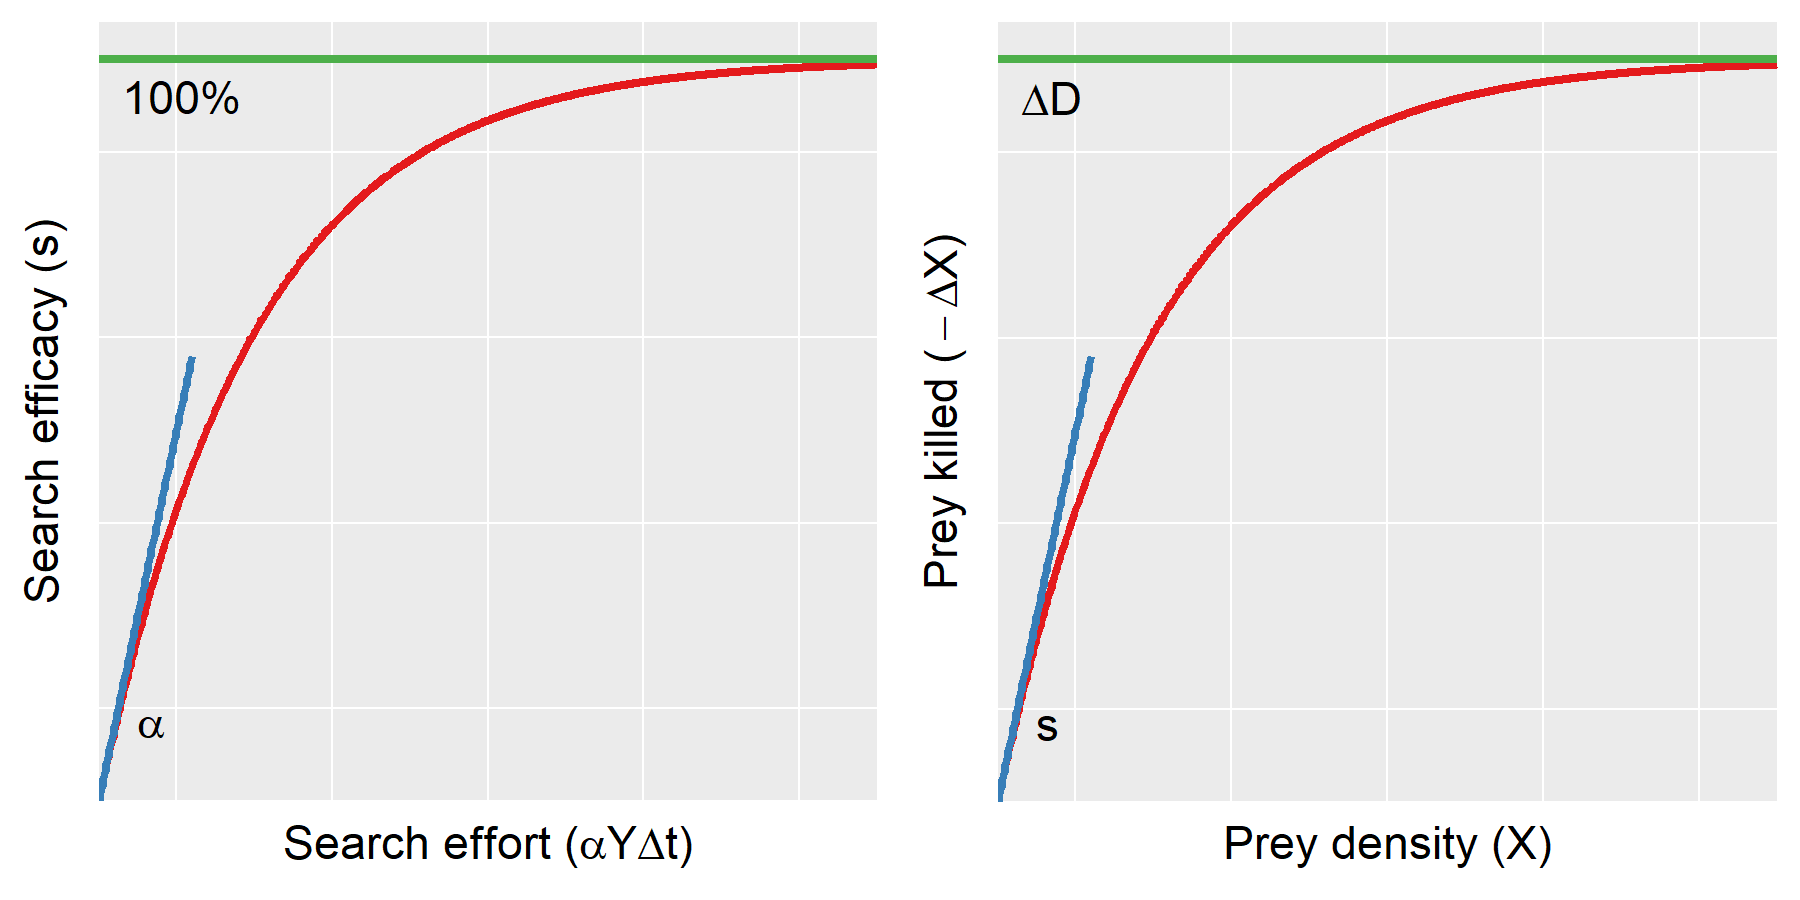
\includegraphics[width=\textwidth]{graphics/func-resp-gb-detail}
\caption{Red curves show search efficacy (left) and functional response (right). Green lines show upper asymptote, 100\% and predator demand ($\Delta D$), respectively. Blue lines show the initial slope of the curves at the origin, attack rate ($\alpha$) and search efficacy ($s$), respectively. Produced by the \filename{\inputfolder/book/func-resp/func-resp-gb-detail.box} script.}
\label{fig:trophic}
\end{figure}

This functional response model \eqref{eq:funcresp} is a form of the Gutierrez-Baumg{\"a}rtner functional response  \citep[][page~71]{Guti96} which is a versatile model, that has been used to describe both predator-prey, parasitoid-host and plant-resource interactions. Depending on the system, the amount of acquired resource ($-\Delta X$) may represent the number of prey killed, number of hosts parasitized, amount of sunlight captured, \etc. It can be seen that prey mortality comes out as $-\Delta X/X\in[\,0;1]$ and the predator's supply/demand ratio as $-\Delta X/\Delta D\in[\,0;1]$. 

Only two parameters need to be determined: the demand rate ($d$) which is genetically determined and can be estimated under optimal conditions and the attack rate ($\alpha$), which is determined by a variety of conditions relating to the biological and physical characteristics of the predator-prey arena. The attack rate is thus an abstraction of many factors which must be estimated (calibrated) during model development.

The functional response model \eqref{eq:funcresp} is implemented in the \code{FunctionalResponse} class which has these inputs:
\begin{itemize}
\item \codenobox{attacker} ($Y$)
\item \codenobox{prey} ($X$)
\item \codenobox{demandGross} ($\Delta D$)
\item \codenobox{attackRate} ($\alpha$)
\item \codenobox{timeStep} ($\Delta t$)
\end{itemize}

\noindent and these outputs:
\begin{itemize}
\item \codenobox{supplyGross} ($-\Delta X$)
\item \codenobox{propPreyAttacked} ($-\Delta X/X$)
\item \codenobox{searchEfficacy} ($s$)
\item \codenobox{sdRatioGross} ($-\Delta X/\Delta D$)
\end{itemize}

The names \code{demandGross} and \code{supplyGross} were chosen to highlight that the amount of prey killed is turned into predator matter (\eg\ in terms of biomass or number of offspring) only at a certain  conversion efficiency. In the Lotka-Volterra model \eqref{eq:lotvol0}, this is accounted for by $\delta$.

The \filenameexplained{book/func-resp/func-resp-bg.box} script demonstrates how to use a \code{FunctionalResponse} box:

\lstset{numbers=left}
\begin{boxscript}
// func-resp-gb.box
Simulation {
  .steps = 100
  .iterations = 3
  Sequence predator {
    .by = "reset"
    .values = (1 2 5)
  }
  Sequence demand {
    .by = "reset"
    .values = (10 20 50)
  }
  Sequence prey {
    .by = "update"
    .min = 0
    .max = 100
  }
  FunctionalResponse funcResp {
    .attacker = predator[value]
    .prey = prey[value]
    .demandGross = demand[value]
    .attackRate = 0.8
  }
  OutputR {
    .end = "func-resp-gb-end.R"
    OutputText {
      .ports = funcResp[*]
    }
  }
}\end{boxscript}
\lstset{numbers=none}

The idea is to show the functional response function \eqref{eq:funcresp} with prey density $X=$ 0 to 100, together with three predator densities $Y=$ 1, 2 and 5, and with fixed rates of demand $d=10$ and attack $\alpha=0.8$. This is achieved by running 3 iterations (line 4) each with 100 steps (line 3).

One \code{Sequence} box (lines 5-8) specifies the three predator densities and another, the corresponding demands (lines 9-12). Their value changes every time the model is \code{reset} (lines 6 and 10). All boxes are reset once at the beginning of each iteration of which we've got three (line 4).

\begin{figure} [ht]
\centering
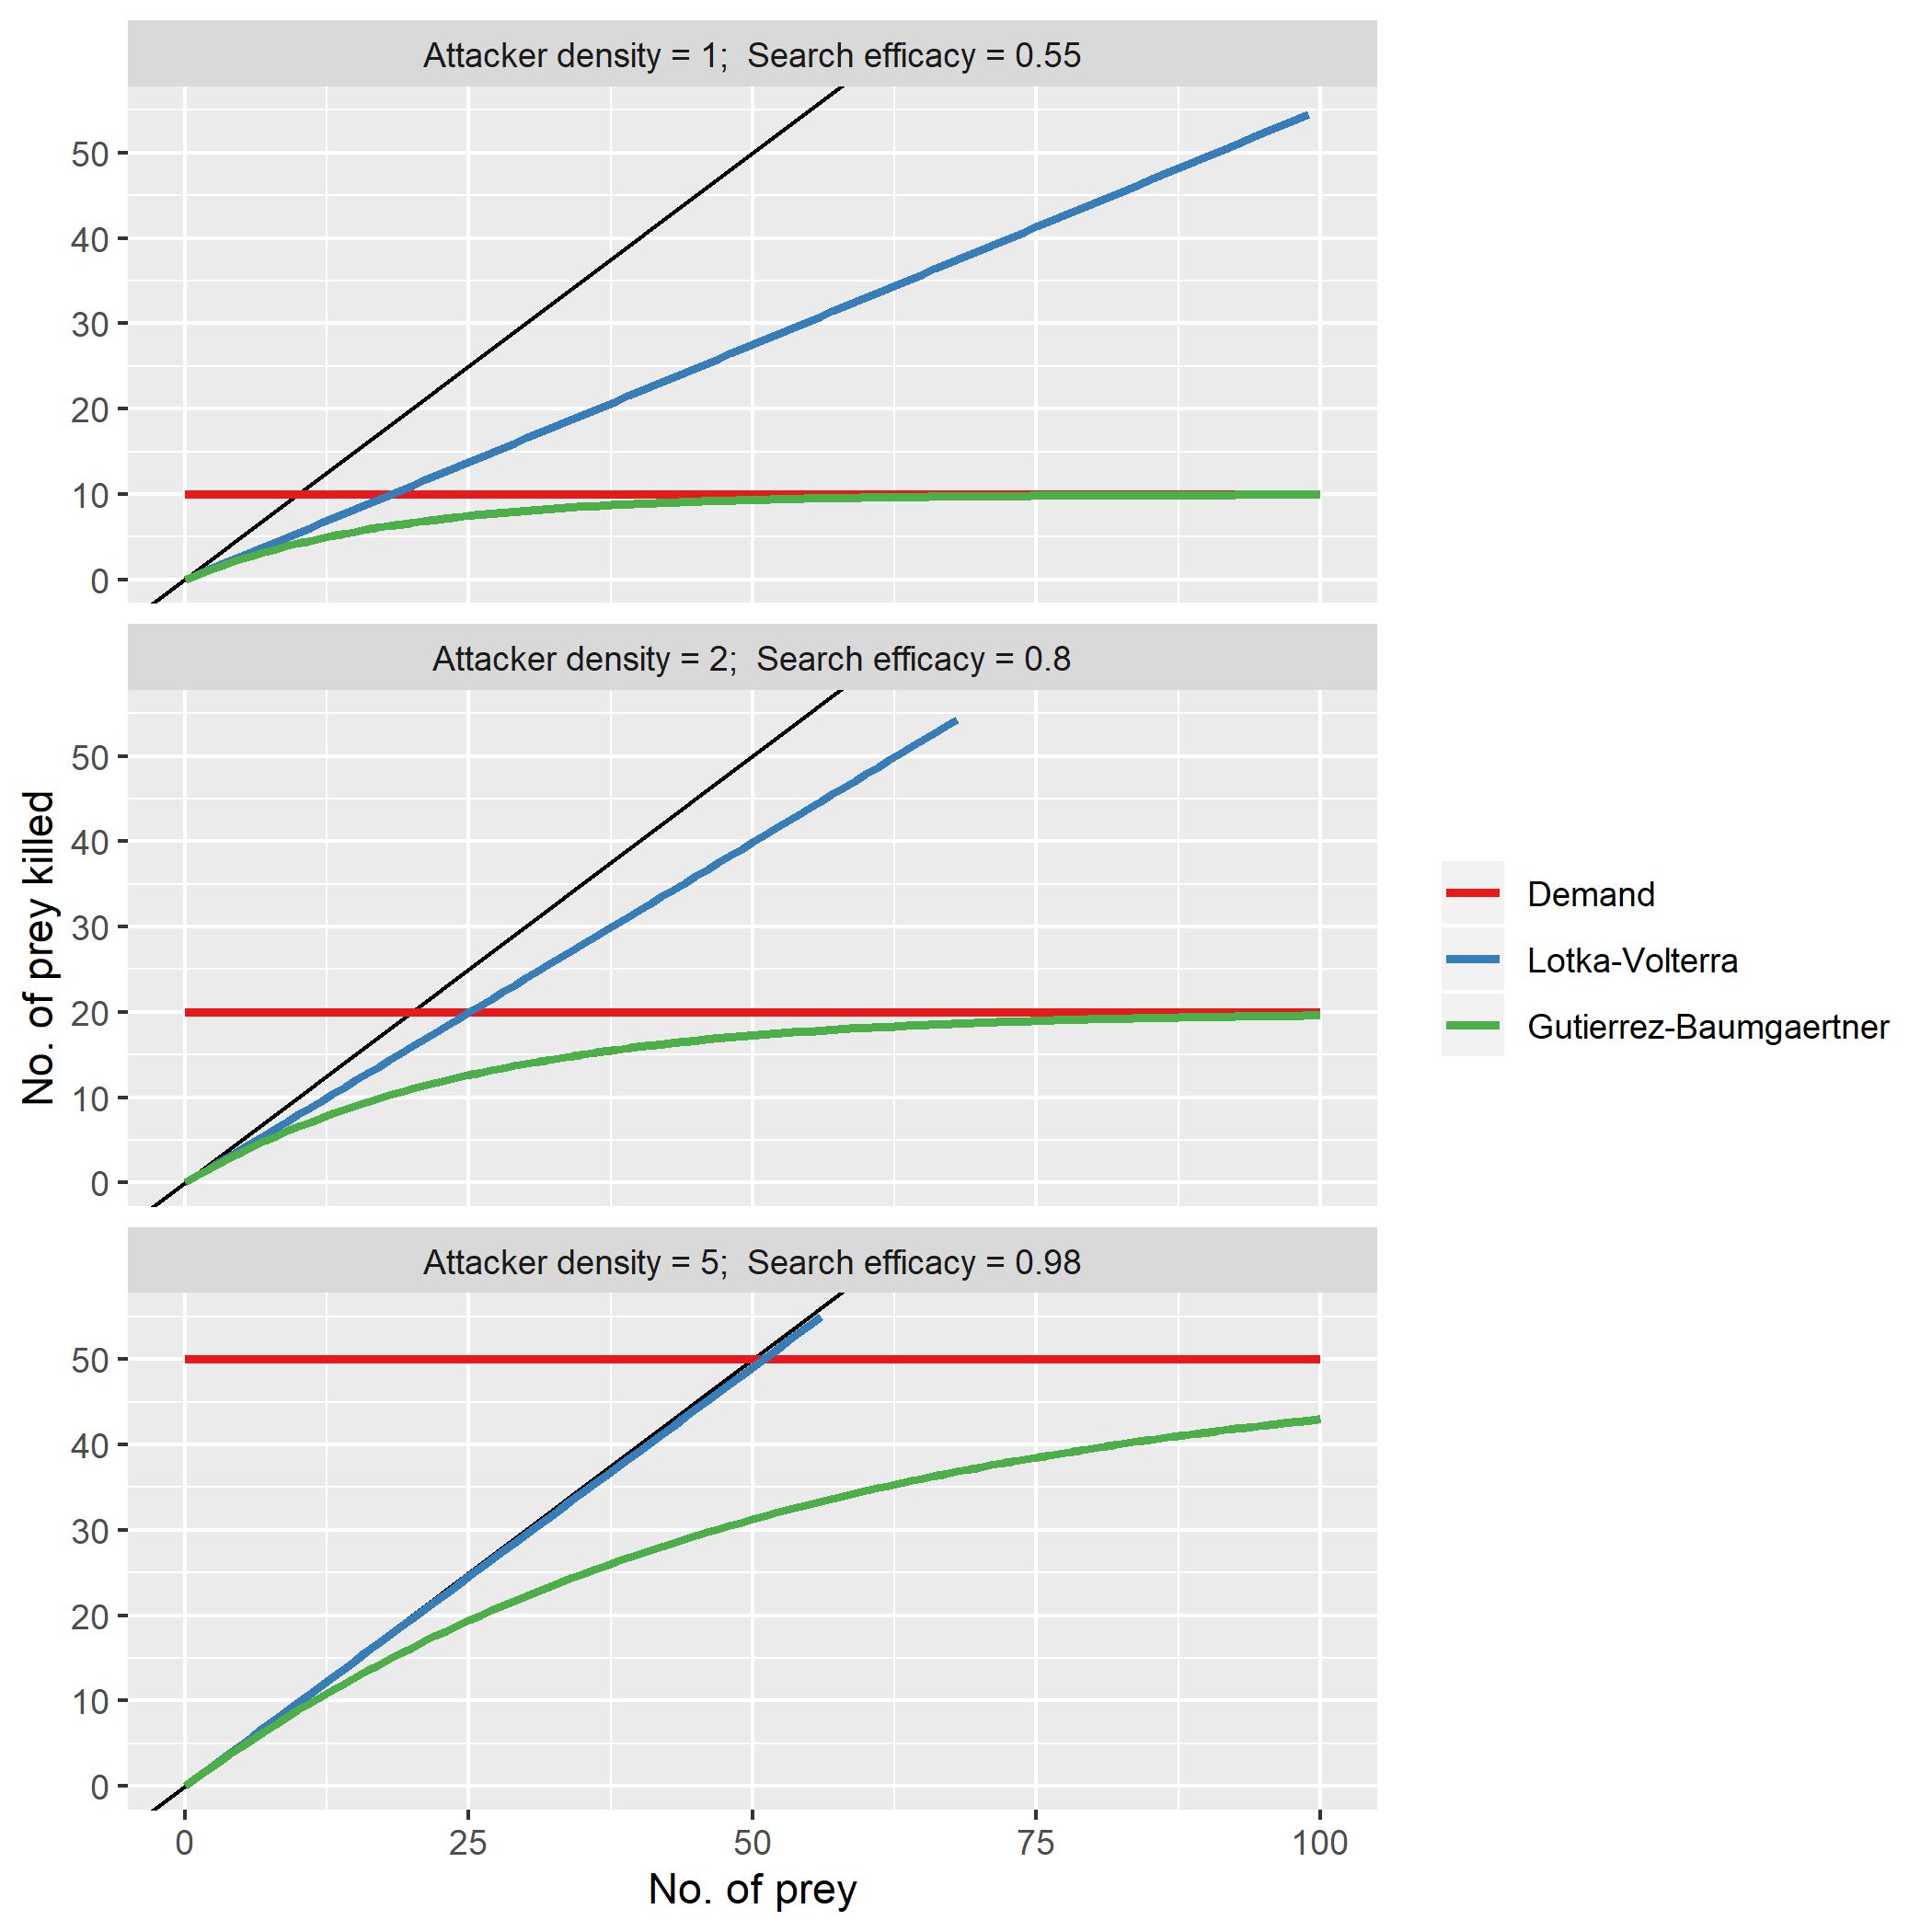
\includegraphics[width=0.9\textwidth]{graphics/func-resp-gb}
\caption{Comparison of the Lotka-Volterra and Gutierrez-Baumg{\"a}rtner functional response models at three predator densities. The black 1:1 line shows $y=x$. Produced by the \filename{\inputfolder/book/func-resp/func-resp-gb.box} script.}
\label{fig:func-resp-gb}
\end{figure}

Yet another \code{Sequence} box (lines 13-17) specifies the range of prey densities by the minimum and maximum values. This sequence of numbers is updated at every \code{update} (line 14) which occurs for every step, of which we've got 100 (line 3).

The search efficacy ($s$) is computed \eqref{eq:lotvol2} from the attack rate ($\alpha$) and the time step ($\Delta t$) which defaults to 1 in the \code{FunctionalResponse} box. You can type \code{help FunctionalResponse} at the \US\ prompt to see the default input values. 

Search efficacy increases with predator density and converges towards the 1:1 black line (\iref{fig:func-resp-gb}). It is shown in the figure by the Lotka-Volterra model, $-\Delta X = sXY$ which coincides with the asymptote of the Gutierrez-Baumg{\"a}rtner model at low prey density \eqref{eq:lotvol2}. 

The Gutierrez-Baumg{\"a}rtner model comes out as superior, as it never exceeds the predator demand, whereas the Lotka-Volterra ignores and overshoots predator demand. Neither model crosses the black 1:1 line, which would imply that more prey was killed than available.


\section{Energy budget}
\label{ch:trophic-energy-budget}

The demand of the predator ($\Delta D$) depends on its current needs for expenditures to respiration, growth and reproduction. Respiration comes in two flavours: the base metabolic rate (proportional to predator biomass and increasing exponentially with temperature) and conversion costs associated with turning prey eaten into predator mass (in terms of bodily growth and reproductive structures and outputs).

We describe these by the energy budget \citep{GutiConc81} which formulates the components that contribute to the gross demand ($\Delta D_{gross}$):

\begin{equation}
\Delta D_{gross} = \dfrac{ \dfrac{\Delta D_{net}}{1-\lambda}+\Delta Z}{1-\beta}\, \text{where}\, \Delta Z = \Delta z Y \Delta t
\label{eq:demandbudget}
\end{equation}
where $\Delta D_{net}$ is the net demand of the predator (\eg\ for assimilation into body growth and reproduction), $\lambda$ is the proportional conversion cost, $z$ is the base respiration rate per predator, and $\beta$ is the egested fraction, \ie\ the fraction of acquired resource going unutilized. $\Delta D_{gross}$ is the gross demand needed to fulfill all requirements for assimilation and expenditures.

The actual amount of acquired resource ($-\Delta X$) is calculated by way of the functional response \eqref{eq:funcresp}. We can re-arrange the demand budget \eqref{eq:demandbudget} to calculate the supply budget by replacing the net demand ($\Delta D_{net}$) with the net supply ($\Delta S_{net}$) and, the gross demand ($\Delta D_{gross}$) with the acquired resource (kill) $-\Delta X$ :

\begin{equation}
\Delta S_{net} =\left[-\Delta X(1-\beta)-\Delta Z\right](1-\lambda)\label{eq:supplybudget}
\end{equation}

The gross supply ($\Delta S_{gross} = -\Delta X$) is what's available to meet the components of the demand budget:

\begin{equation}
  \begin{aligned}
    \Delta S_{gross} &= S_{egest} + S_{resp} + S_{conv} + S_{net} \\
    \Delta S_{egest} &= -\beta \Delta X \\
    \Delta S_{resp}  &= \Delta Z \\
    \Delta S_{conv}  &= \lambda(-\Delta X - \Delta S_{egest} - \Delta S_{resp}) \\
    \Delta S_{net}   &= -\Delta X - \Delta S_{egest} - \Delta S_{resp} - \Delta S_{conv}
  \end{aligned} \label{eq:supplyallocation}
\end{equation}

Note that the net supply $\Delta S_{net}$ available for predator assimilation will be negative, in case the demand for base respiration ($\Delta Z$) cannot be met by a sufficient supply, \ie\ the predator is starving. Depending on the concrete organism, you must decide how to handle this case in your model.

\begin{figure} [hb]
\centering
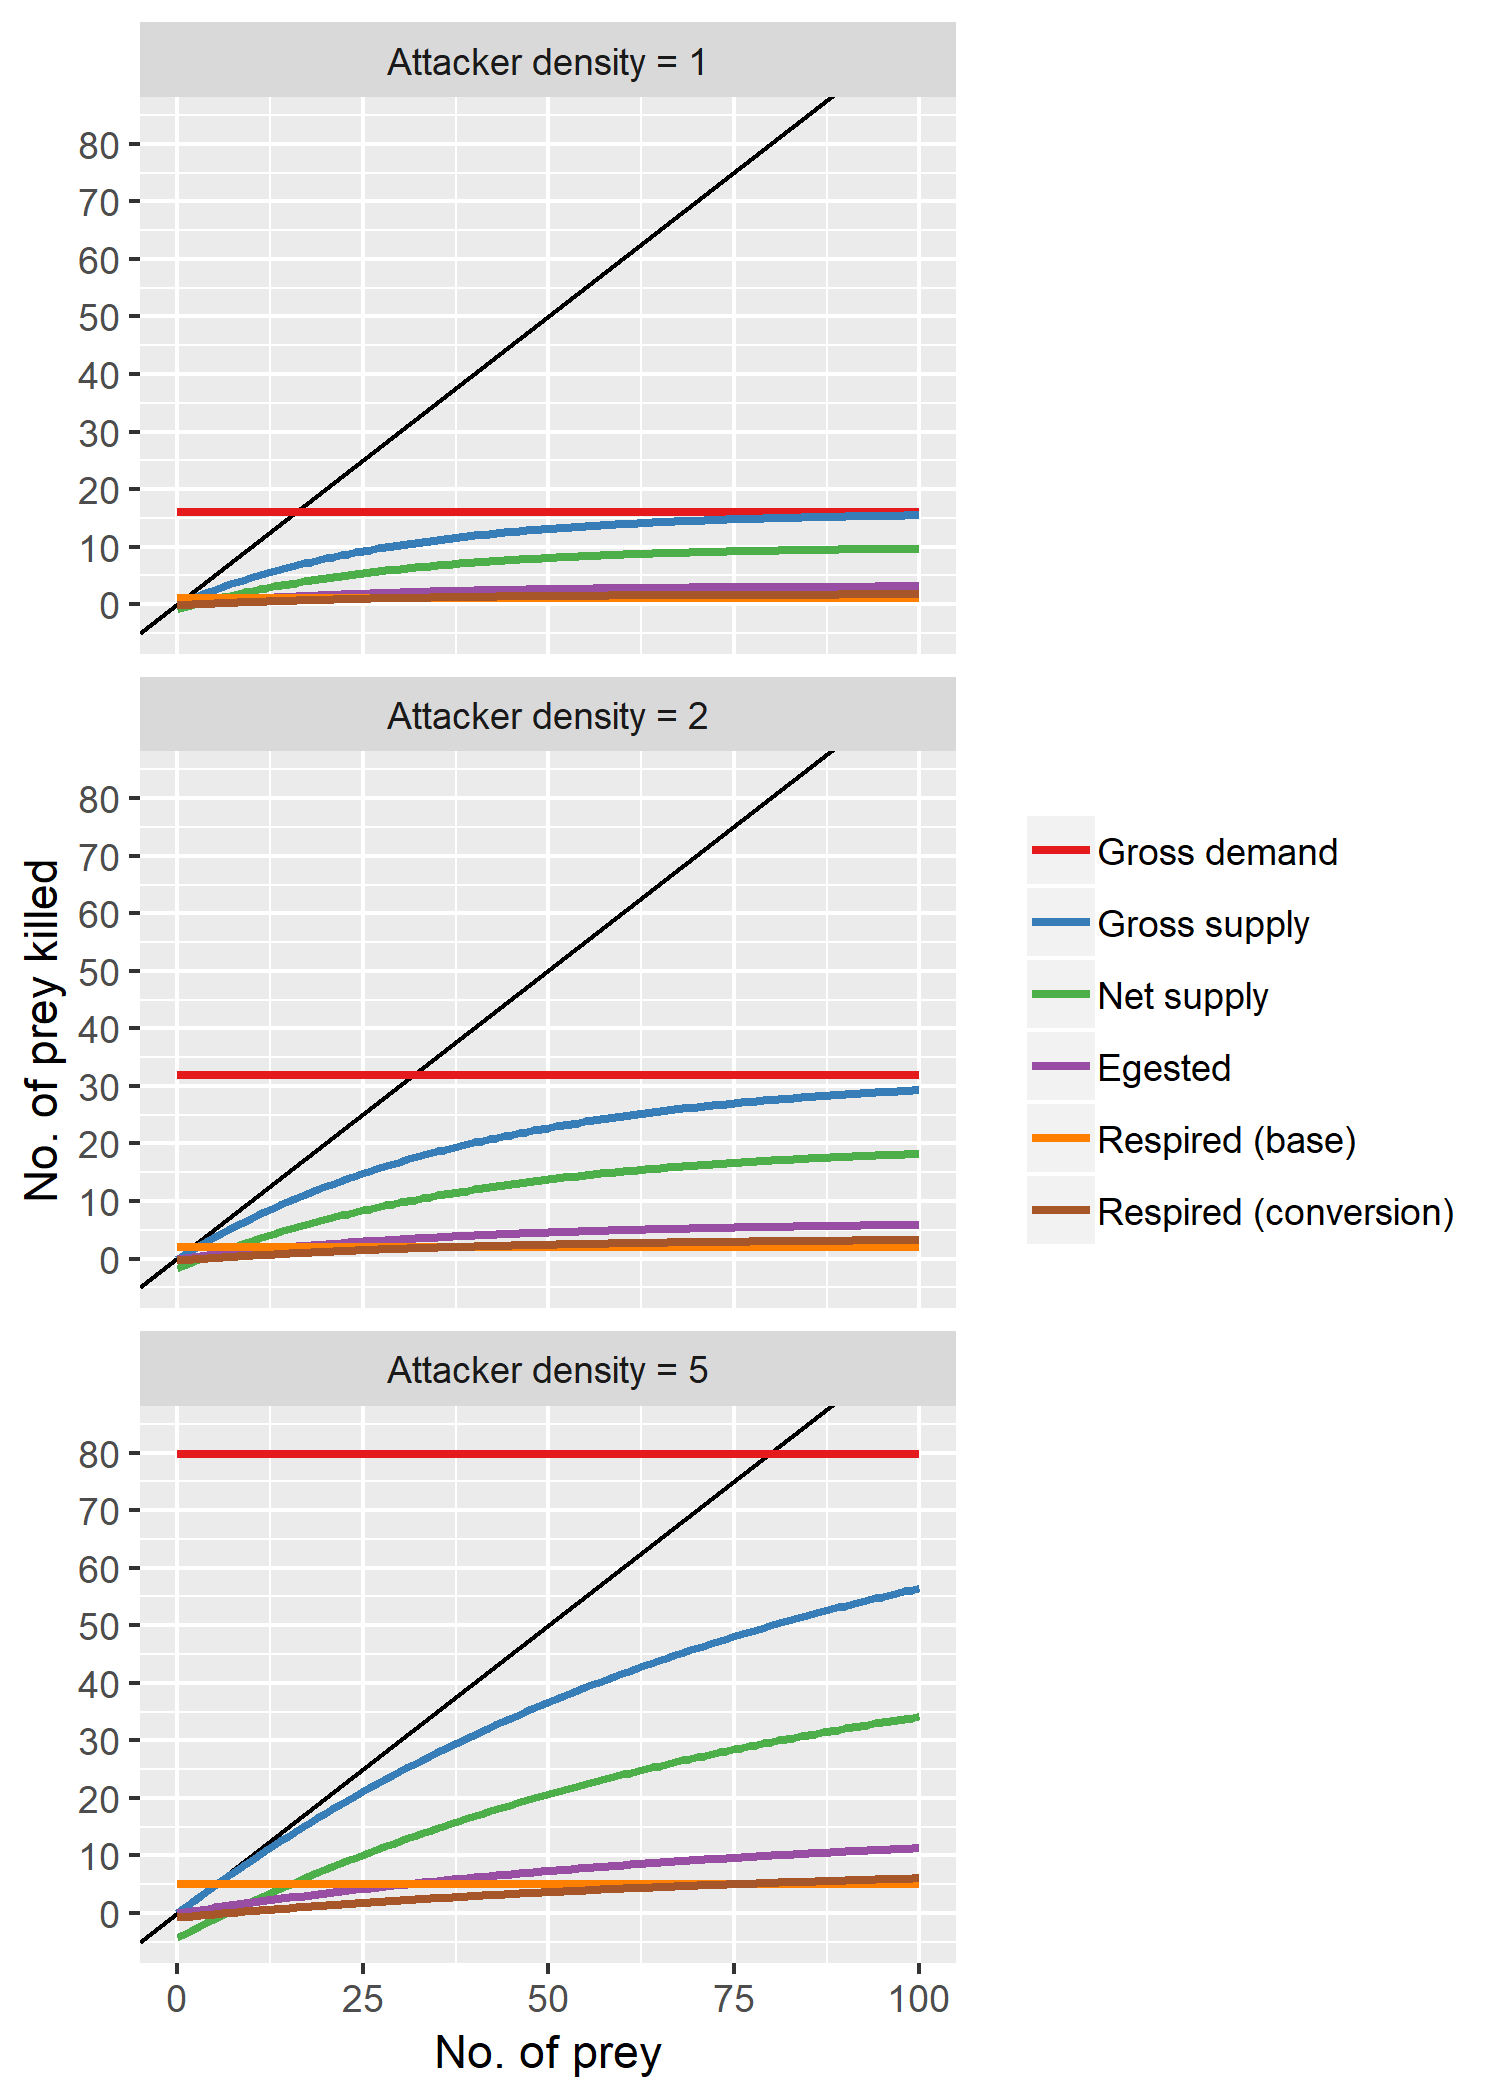
\includegraphics[width=0.9\textwidth]{graphics/func-resp-energy-budget}
\caption{ The predator's energy budget at three predator densities. The black 1:1 line shows $y=x$. Produced by the \filename{\inputfolder/book/func-resp/func-resp-energy-budget.box} script.}
\label{fig:func-resp-energy-budget}
\end{figure}

You may find that for a particular system, the generic energy budget of \cref{eq:demandbudget,eq:supplybudget,eq:supplyallocation} is not sufficient. Sometimes, a more detailed physiological model is necessary to model the energy budget, for instance, to include energy reserves in the predator.

The box script below follows the previous example, only now the predator's energy budget is included:

\lstset{numbers=left}
\begin{boxscript}
// func-resp-energy-budget.box
Simulation {
  .steps = 100
  .iterations = 3
  Sequence predator {
    .by = "reset"
    .values = (1 2 5)
  }
  Sequence demand {
    .by = "reset"
    .values = (10 20 50)
  }
  Sequence respiration {
    .by = "reset"
    .values = (1 2 5)
  }
  Sequence prey {
    .by = "update"
    .min = 0
    .max = 100
  }
  Box param {
    +conversionCost = 0.15
    +egested = 0.2
  }
  DemandBudget demandBudget {
    .demandNet = demand[value]
    .demandResp = respiration[value]
    .conversionCost = param[conversionCost]
    .egested = param[egested]
  }
  FunctionalResponse funcResp {
    .attacker = predator[value]
    .prey = prey[value]
    .demandGross = demandBudget[demandGross]
    .attackRate = 0.8
  }
  SupplyBudget supplyBudget {
    .supplyGross = funcResp[supplyGross]
    .demandNet = demand[value]
    .demandResp = respiration[value]
    .conversionCost = param[conversionCost]
    .egested = param[egested]
  }
  OutputR {
    .end = "func-resp-energy-budget-end.R"
    OutputText {
      .ports = (funcResp[attacker] funcResp[prey] 
                funcResp[demandGross] supplyBudget[*])
    }
  }
} \end{boxscript}
\lstset{numbers=none}

Four parameters are used both in the demand and supply budgets. For convenience and to guard against inconsistency, we create two additional inputs to set thes parameter values for $\beta$ and $\lambda$ (lines 23-34). They are both inside a \code{param} box which has no other function than holding these parameters.

The \code{DemandBudget} (lines 26-31) implements the energy budget \eqref{eq:demandbudget} with these inputs:
\begin{itemize}
\item \codenobox{demandNet} ($\Delta D_{net}$)
\item \codenobox{demandResp} ($z$)
\item \codenobox{conversionCost} ($\lambda$)
\item \codenobox{egested} ($\beta$)
\end{itemize}

\noindent which result in one output:
\begin{itemize}
\item \codenobox{demandGross} ($\Delta D_{gross}$)
\end{itemize}

This \code{demandGross} output enters the functional response (line 35) which computes the gross supply \code{supplyGross}.

The \code{SupplyBudget} (lines 38-44) implements the energy budget \eqref{eq:supplybudget}, in terms of how the gross supply is distributed among the expenditures. It shares four of its inputs with the \code{DemandBudget}. In addition it needs to know the gross supply (line 39). Its outputs are

\begin{itemize}
\item \codenobox{supplyNet} ($\Delta S_{net}$)
\item \codenobox{egestedAmount} ($\Delta S_{egest}$)
\item \codenobox{conversionCostAmount} ($\Delta S_{conv}$)
\item \codenobox{sdRatioNet} ($-\Delta S_{net}/\Delta D_{net}$)
\end{itemize}

The output (\iref{fig:func-resp-energy-budget}) shows that for $Y=5$, for example, the gross demand $\Delta D_{gross}=79.8$ prey turns out quite larger than the net demand $\Delta D_{net}=10$ prey (\iref{fig:func-resp-gb}). Thus is due to the expenditures defined by the energy budget \eqref{eq:demandbudget}.

The gross supply is obtained by way of the \GB\ functional response \eqref{eq:funcresp}. Part of the gross supply is assimilated (net supply) while the rest is allocated among the different expenditures (\iref{fig:func-resp-energy-budget}). Note that at high attacker density and low prey density, the base respiration may exceed the the supply. This shows as net supply becoming negative. If this script were part of a larger model, a decision would have to be taken how to incorporate this situation in the model, \eg\ by increased predator mortality.

%\afterpage{\clearpage}
\FloatBarrier
\section{The super functional response}
\label{ch:super-functional-response}
I suggest the concept \concept{super functional response} to describe the case in which a resource individual (the host) may suffer several attacks from the attacker population (the super attacker). The concept covers superparasitism, which refers to the habit of some parasitoid species to parasitise a host even if it has already been parasitised by the same species. Depending on the specific biology, one or more parasitoids may develop from such a superparasitised host. Likewise, bloodsucking insects may attack the same host many times. The host is usually unaffected (unless the attacker is an infectious vector) but the attacker is rewarded by a blood meal. 

Unlike the predator-prey functional response (\iref{ch:trophic-functional-response}), the super functional response may lead to the number of attacks being larger than the number of hosts. Note that in functional response parlance, an attack always refers to a successful attack. Instead of each host being attacked 0 or 1 times, it can be attacked any number of times. If hosts are attacked at random, the probability of being attacked $n$ times follows a Poisson distribution $P_{\lambda}(n)$ which is described by only one parameter $\lambda$: the average number of attacks per host. Notably, the number of hosts not attacked is $P_{\lambda}(0)=e^{-\lambda}$.

To derive a model for the super functional response, we begin with the \GB\ functional response for predators \eqref{eq:funcresp}

\begin{equation}
-\Delta X = \Delta D \left[1-exp\left(\frac{-sX}{\Delta D}\right)\right] \label{eq:super1}
\end{equation}

\begin{equation}
  \Delta D = dY\Delta t \label{eq:super2}
\end{equation}

\begin{equation}
  s = 1-exp(-\alpha Y \Delta t) \label{eq:super3}
\end{equation}

\noindent in which \eqref{eq:super1} limits the number of prey killed to the predator's demand, and \eqref{eq:super3} limits the number of prey killed to the number of prey available. 

For a super attacker, however, the demand is in units of attack numbers not in units of host numbers. Consequently, the outcome of \eqref{eq:super1} must be the number of attacks not, as for a predator, the number of prey killed. A super attacker is demand-limited, just like a predator; thus \eqref{eq:super2} still applies. The search efficacy, however, is not limited to the number of hosts. Hence, for a super attacker, we need to reformulate both \eqref{eq:super1} and \eqref{eq:super3}:

\begin{equation}
  \Delta S_a = \Delta D \left[1-exp\left\{\frac{-sX}{\Delta D}\right\}\right] \label{eq:super4}
\end{equation}

\begin{equation}
  s = \alpha Y \Delta t \label{eq:super5}
\end{equation}

Here, we introduce $\Delta S_a$ for the supply in terms of number of attacks while the simple, linear expression for search efficacy \eqref{eq:super5} takes us back to the Lotka-Volterra equation \eqref{eq:lotvol1}. 

The limits of \eqref{eq:super4} are

\begin{equation}
  \begin{aligned}
    \Delta S_a \rightarrow \alpha XY \Delta t\quad &\text{for}\quad X\rightarrow 0 \lor Y\rightarrow 0 \\
    \Delta S_a \rightarrow \Delta D\quad           &\text{for}\quad X\rightarrow \infty
  \end{aligned} \label{eq:limsa}
\end{equation}

\noindent which means that the response will curve gradually away from the linear Lotka-Volterra response towards the demand as host density ($X$) increases.

The average number of attacks per host is 

\begin{equation}
  \lambda = \frac{\Delta S_a}{X} 
\end{equation}

\noindent which we can combine with \eqref{eq:super2}, \eqref{eq:super4} and \eqref{eq:super5} to get

\begin{equation}
  \lambda = \frac{\Delta D}{X} \left[1-exp\left\{\frac{-\alpha X}{d}\right\}\right] 
\end{equation}

Note how the term $Y \Delta t$ cancelled out in the exponentiated fraction. From this follows the proportion of hosts attacked ($P_{X_a}$), as one minus the zero term of the Poisson distribution,

\begin{equation}
  P_{X_a} = 1 - exp \left\{-\frac{\Delta D}{X} \left[1-exp\left\{\frac{-\alpha X}{d}\right\}\right] \right\}
\end{equation}

\noindent and finally the number of hosts attacked

\begin{equation}
  \Delta X_a = \left[ 1 - exp \left\{-\frac{\Delta D}{X} \left[1-exp\left\{\frac{-\alpha X}{d}\right\}\right] \right\} \right] X \label{eq:frazer-gilbert}
\end{equation}

This impressive equation is the Frazer-Gilbert functional response model \citep{FrazerGilbert} also credited by \citet{GutiConc81}. The limits of it are

\begin{equation}
  \begin{aligned}
    \Delta X_a \rightarrow X\quad        &\text{for}\quad X\rightarrow 0 \\
    \Delta X_a \rightarrow \Delta D\quad &\text{for}\quad X\rightarrow \infty
  \end{aligned}
\end{equation}

\begin{figure} [ht]
\centering
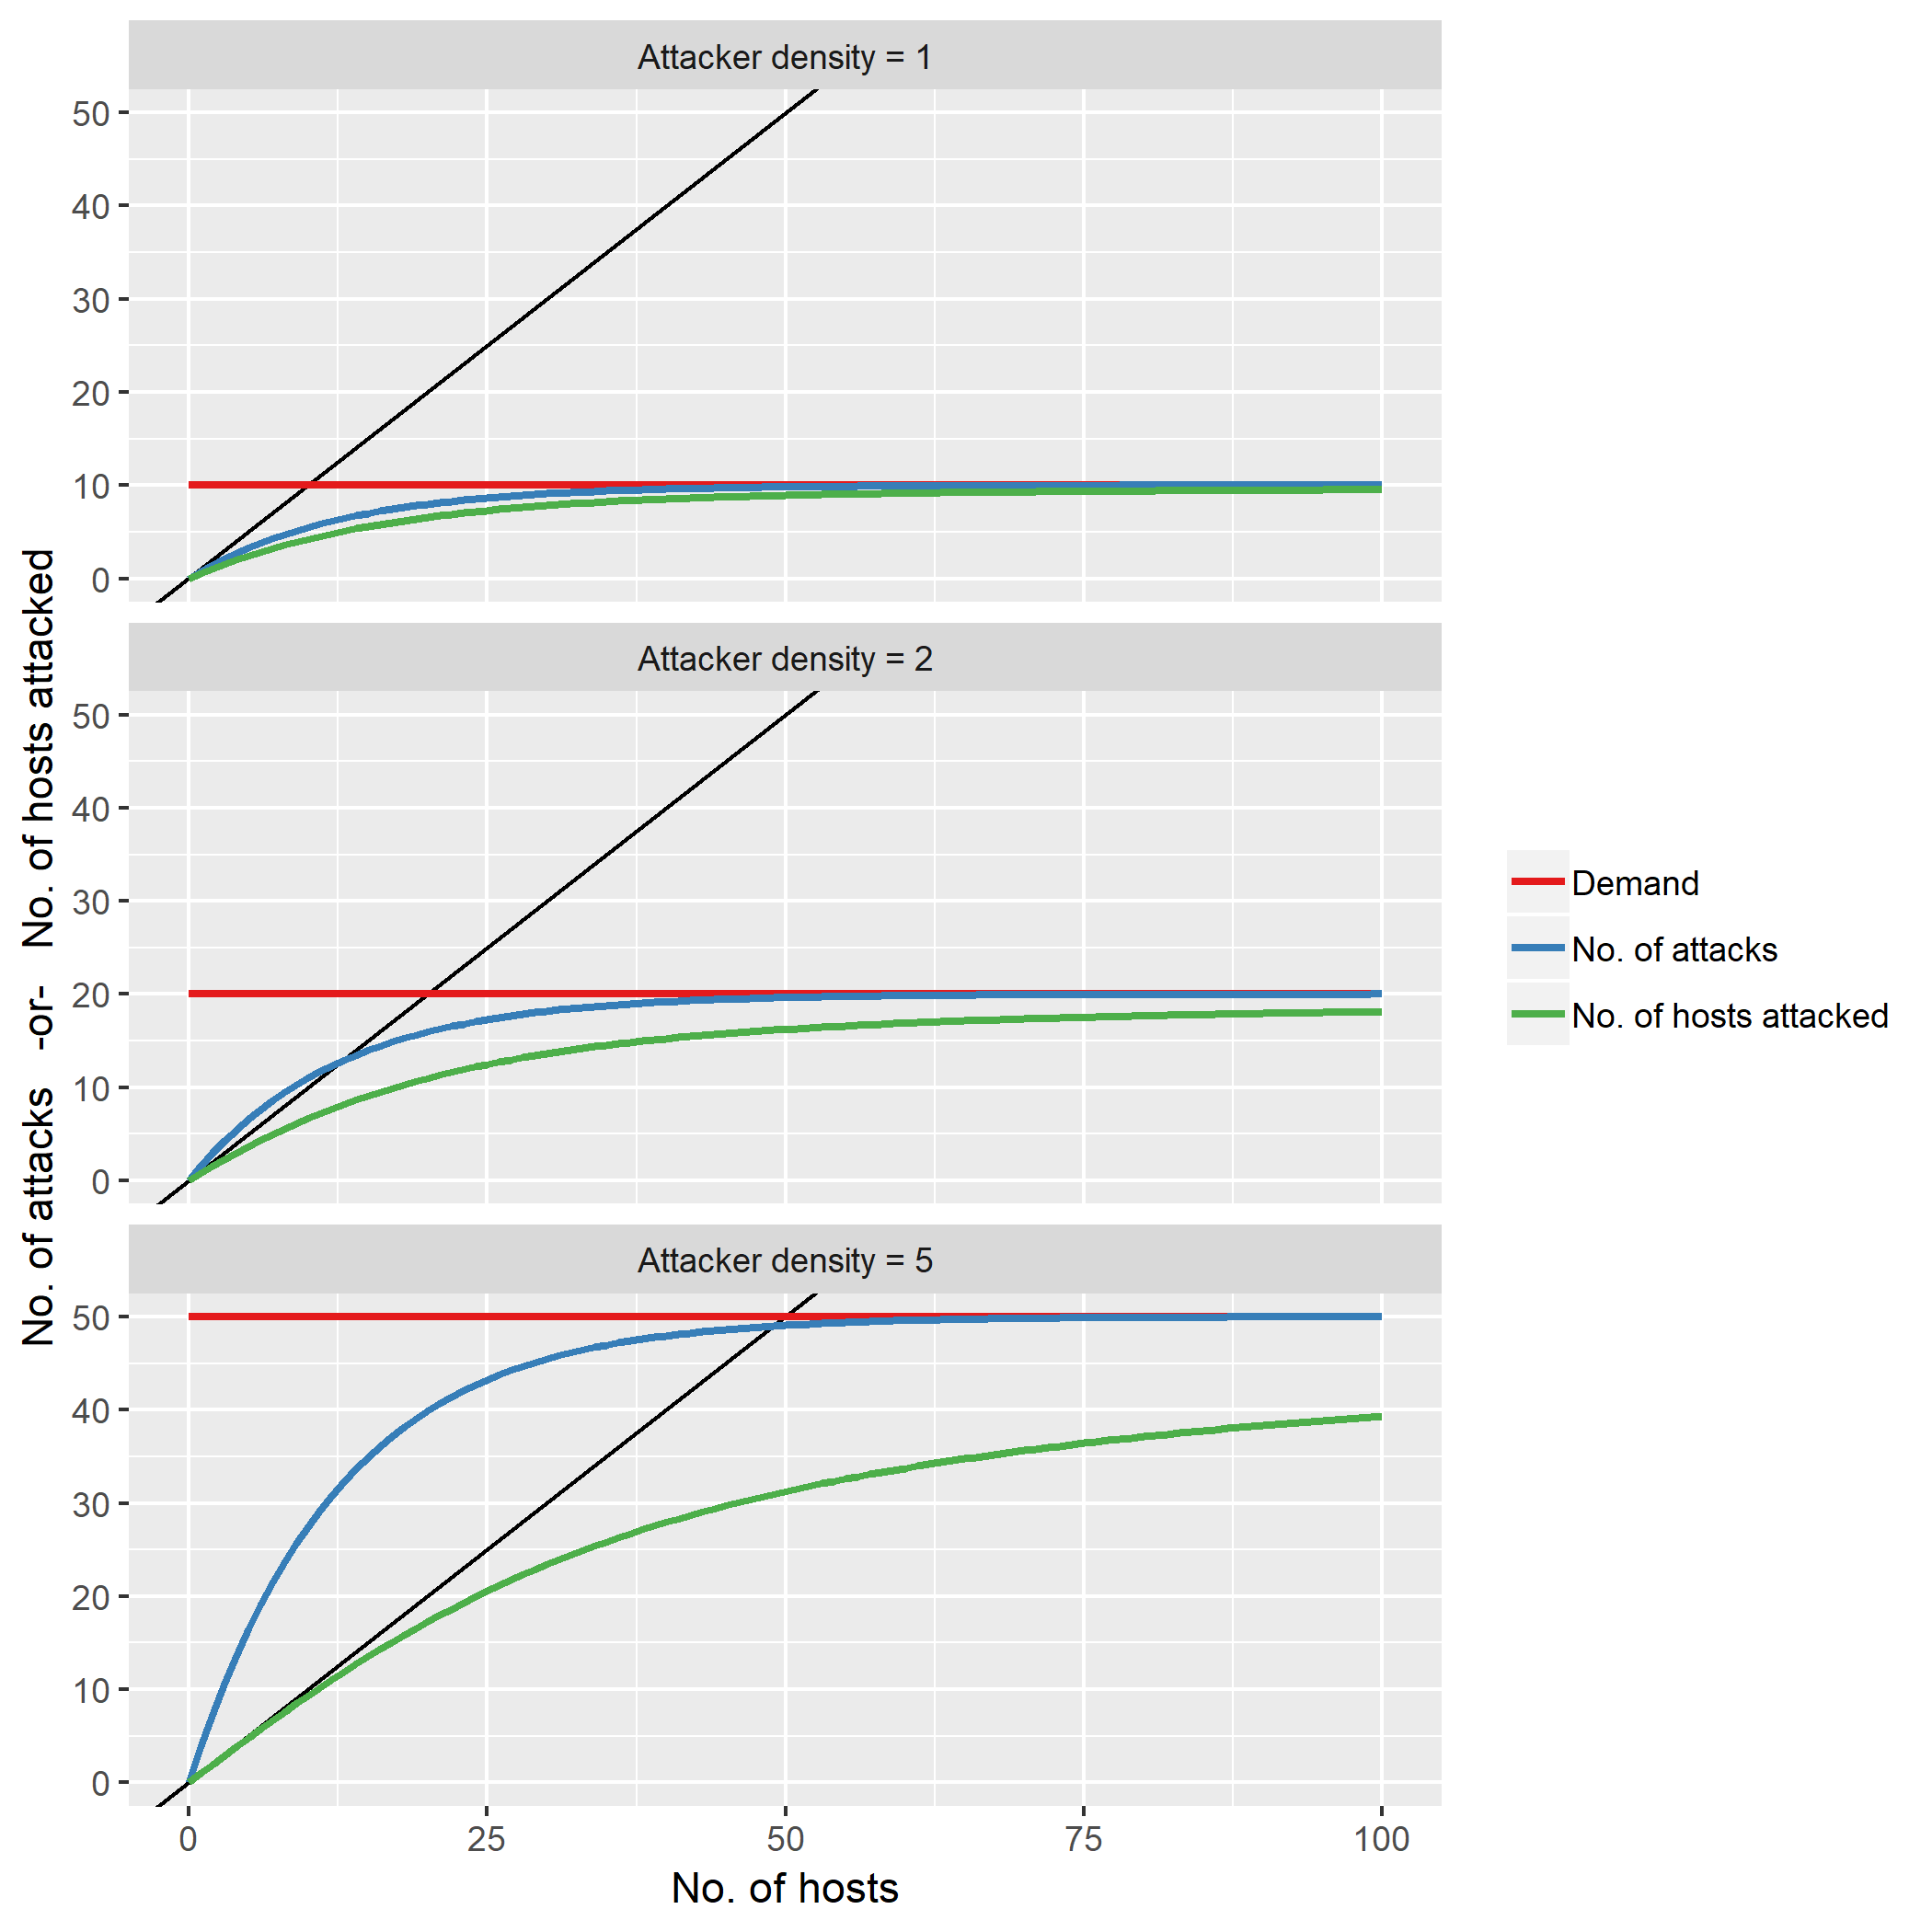
\includegraphics[width=0.9\textwidth]{graphics/func-resp-fg}
\caption{Comparison of two outcomes of the Frazer-Gilbert functional response model, the number of attacks \vs\ the number of hosts attacked. The black 1:1 line shows $y=x$. Produced by the \filename{\inputfolder/book/func-resp/func-resp-fg.box} script.}
\label{fig:func-resp-fg}
\end{figure}

This means that at low host density ($X$), all hosts will tend to be attacked. At high host density, not only will the number of attacks ($\Delta S_a$) approach the demand ($\Delta D$) \eqref{eq:limsa}, so will the number of attacked hosts ($\Delta X_a$). Thus we have

\begin{equation}
  \frac{\Delta S_a}{\Delta X_a} \rightarrow 1\quad \text{for}\quad X\rightarrow \infty
\end{equation}

In other words, the number of attacks per attacked host will converge towards one at high host density. Or, put more straightforwardly, those hosts that were attacked will tend to have been attacked only once. This corresponds to a maximum spread of the attacks. When there are many hosts relative to the number of attacks delivered, the chances of getting attacked more than once tapers off as the host population increases.

In epidemics modelling, it can be usefull to know the proportion of successfull attackers ($P_{Y_a}$). Seing that the average number of attacks per attacker is

\begin{equation*}
  \frac{\Delta S_a}{Y}
\end{equation*}

\noindent and again applying the zero term of the Possion distribution, we get 

\begin{equation}
  P_{Y_a} = 1 - exp\left(-\frac{\Delta S_a}{Y}\right)
\end{equation}


The super functional response model \eqref{eq:frazer-gilbert} is implemented in the \code{SuperFunctionalResponse} class which has these inputs:

\begin{itemize}
\item \codenobox{attacker} ($Y$)
\item \codenobox{host} ($X$)
\item \codenobox{demand} ($\Delta D$)
\item \codenobox{attackRate} ($\alpha$)
\item \codenobox{timeStep} ($\Delta t$)
\end{itemize}

\noindent and these outputs:
\begin{itemize}
\item \codenobox{supply} ($\Delta S_a$)
\item \codenobox{hostsAttacked} ($\Delta X_a$)
\item \codenobox{propHostsAttacked} ($P_{X_a}$)
\item \codenobox{propAttackersAttacked} ($P_{Y_a}$)
\item \codenobox{sdRatio} ($\Delta S_a/\Delta D$)
\end{itemize}

A test run of the model (\iref{fig:func-resp-fg}) shows that, as expected, the number of attacks is limited by the demand but not by the number of hosts (blue curve superceeding the 1:1 line). And, that the number of hosts attacked is limited both by the number of hosts available (green curve staying below 1:1 line) and by the demand. 

\begin{figure} [ht]
\centering
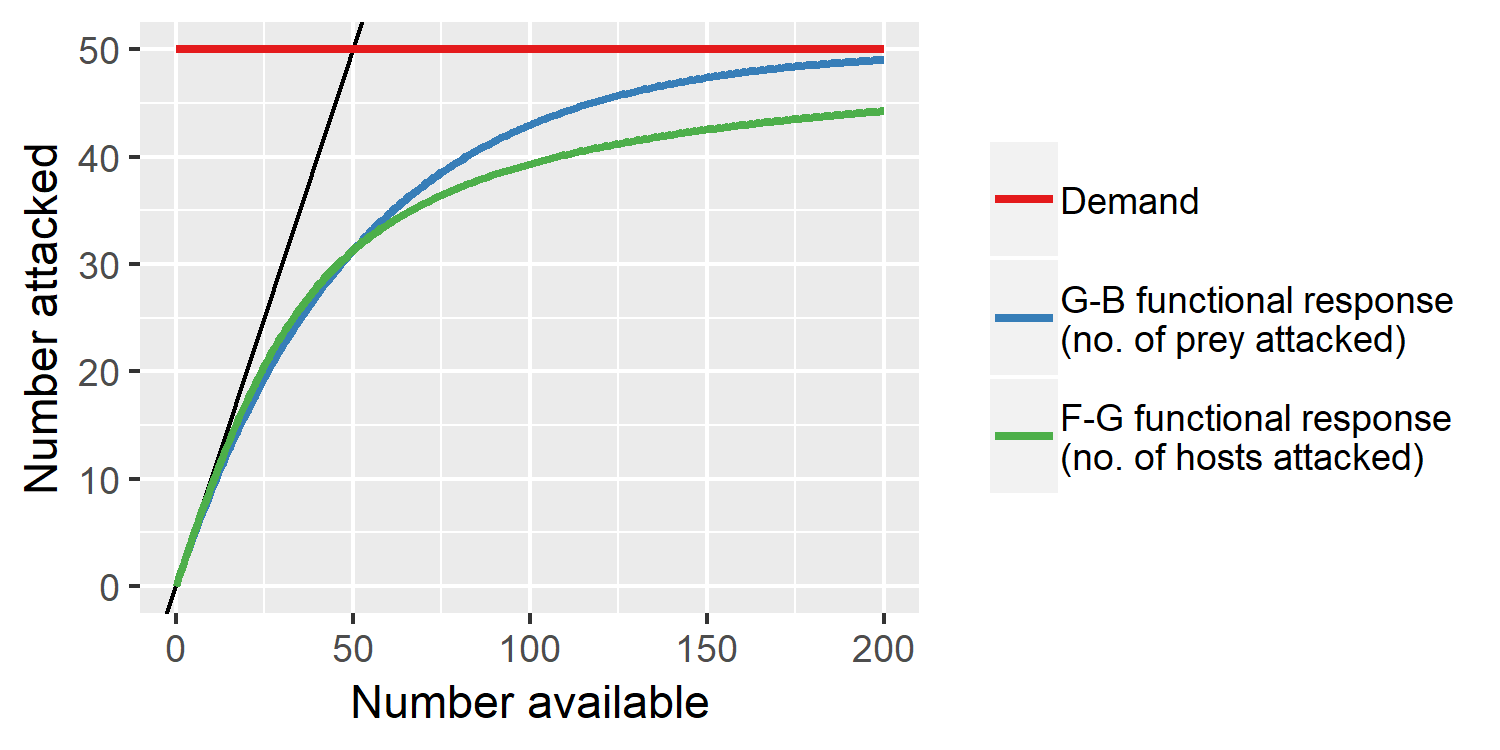
\includegraphics[width=0.9\textwidth]{graphics/func-resp-gb-fg}
\caption{Comparison of the \GB\ \vs\ the Frazer-Gilbert functional response model, both with $Y=5$, $\alpha=0.8$ and $\d=5$. The black 1:1 line shows $y=x$. Produced by the \filename{\inputfolder/book/func-resp/func-resp-gb-fg.box} script.}
\label{fig:func-resp-gb-fg}
\end{figure}

Finally, we compare the two functional response models when given the same parameter values (\iref{fig:func-resp-gb-fg}). We can see that the \GB\ model saturates more quickly to prey density than the Frazer-Gilbert model saturates to host density. This is an effect of the Poisson-distributed attacks that we attacked in the Frazer-Gilbert model. Thereby, we assumed that attacks occurs at random. In reality, they are more likely to be clumped due to the typical behaviour of hosts and, say, mosquitoes. We could include that by choosing the zero term of a clumped distribution, such as the negative binomial, $P_{\lambda,k}(0)$ with mean $\lambda$ and clumpedness parameter $k$. However, this would give us the burden of yet another difficult-to-estimate parameter, namely $k$. Remember that we already have one difficult parameter, which is the attack rate ($\alpha$). Extending the model with one for clumpledness would push our model onto thin ice -- or maybe into interesting waters?.

\FloatBarrier
\section{Population dynamics}
\subsection{Predator-prey}

We will use the \filename{\inputfolder/book/butterfly4.box} script as a starting point for the prey sub-model in a predator-prey model. We create the predator as an egg predator with a life cycle  similar to its prey. The listing shows oly parts of the  \filename{\inputfolder/book/func-resp/func-rep-pred-prey.box} script with a focus on the predator-prey interaction:

\lstset{numbers=left}
\begin{boxscript}
// func-resp-pred-prey.box
Simulation sim {
  .steps = 365
  :
  Box butterfly {
    Stage egg {
      .initial = 100 
      .inflow = ../adult/oviposition[outflow] 
      .duration = 140
      .timeStep = ./time[value]
      .instantLossRate = predation/funcResp[propPreyAttacked]
      :
    }
    Stage larva {
    :
    }
    Stage pupa {
    :
    }
    Box adult {
    :
    }
  }
  Box predator {
    Stage egg {
      .initial = 100 
      .inflow = ../predation/supplyBudget[supplyNet]
      .duration = 140
      .timeStep = ./time[value]
      :
    }
    Stage larva {
    :
    }
    Stage pupa {
    :
    }
    Stage adult {
      .inflow = ../pupa[outflow]
      .duration = 60
      .timeStep = 1
    }
    Stage ovipositionDemand {
      .inflow = ../pupa[outflow]
      .duration = 60
      .timeStep = 1
      .growthFactor = 30
    }
    Box predation {
      Box budget {
        +demandNet = ../../ovipositionDemand[outflow]
        +conversionCost = 0.25
      }
      DemandBudget demandBudget {
        .demandNet = ../budget[demandNet]
        .conversionCost = ../budget[conversionCost]
      }
      FunctionalResponse funcResp {
        .attacker = ../../adult[content]
        .prey = butterfly/egg[content]
        .demandGross = ../demandBudget[demandGross]
        .attackRate = 0.8
      }
      SupplyBudget supplyBudget {
        .demandNet = ../budget[demandNet]
        .conversionCost = ../budget[conversionCost]
        .supplyGross = ../funcResp[supplyGross]
      }
    }
  }
  OutputR {
  :
  }
}
\end{boxscript}
\lstset{numbers=none}

For simplicity, we let the model run for a year only (line 3). Butterfly eggs have a  mortality (line 11) determined by \code{propPreyAttacked} computed by the functional response model (lines 58-63). 

The fecundity of the predator depends on the supply of prey eggs. Hence, the \code{inflow} into the predator egg stage (line 27) comes from the \code{supplyNet} output of the supply energy budget (lines 64-68).

The fecundity under optimal conditions (\ie\ food-unlimited) is formulated as an oviposition demand (lines 43-48) with a net reproductive rate of 30 (line 47). The number of eggs potentially laid on a day enters the demand budget (lines 54-57) as net demand (line 55). The budget adds an expenditure of 0.25 going into conversion costs, \ie\ every prey egg eaten will result in 0.75 predator eggs. Since the same value should be used both in the demand and supply budgets (lines 56 and 66), \code{conversionCost} is defined as a blind port (line 52).

The outcome of the demand budget enters as the gross demand (\ie\ for prey eggs) (line 61)in the functional response (lines 58-63). An attack rate of 0.8 is assumed (line 62). The outcome of the functional response enters as the gross supply (line 67) into the supply budget (lines 64-68), which is the source for the net supply (\ie\ converted into predator eggs) entering as inflow into the egg stage (line 27).

The simulation output (\iref{fig:func-resp-pred-prey}) shows that most of the 4,000 (around 3,989) eggs produced by the butterfly population were eaten by the predator, resulting in nearly 3,000 (around 2,992) predator eggs. The difference being caused by the conversion cost, $\lambda=0.25$. Correspondingly, the ratio between eggs eaten and eggs laid is 2,992/3,989=0.75. Only around 11 butterfly eggs survived. The final population densities were extracted at the R prompt by \code{tail(sim)}.

\begin{figure} 
\centering
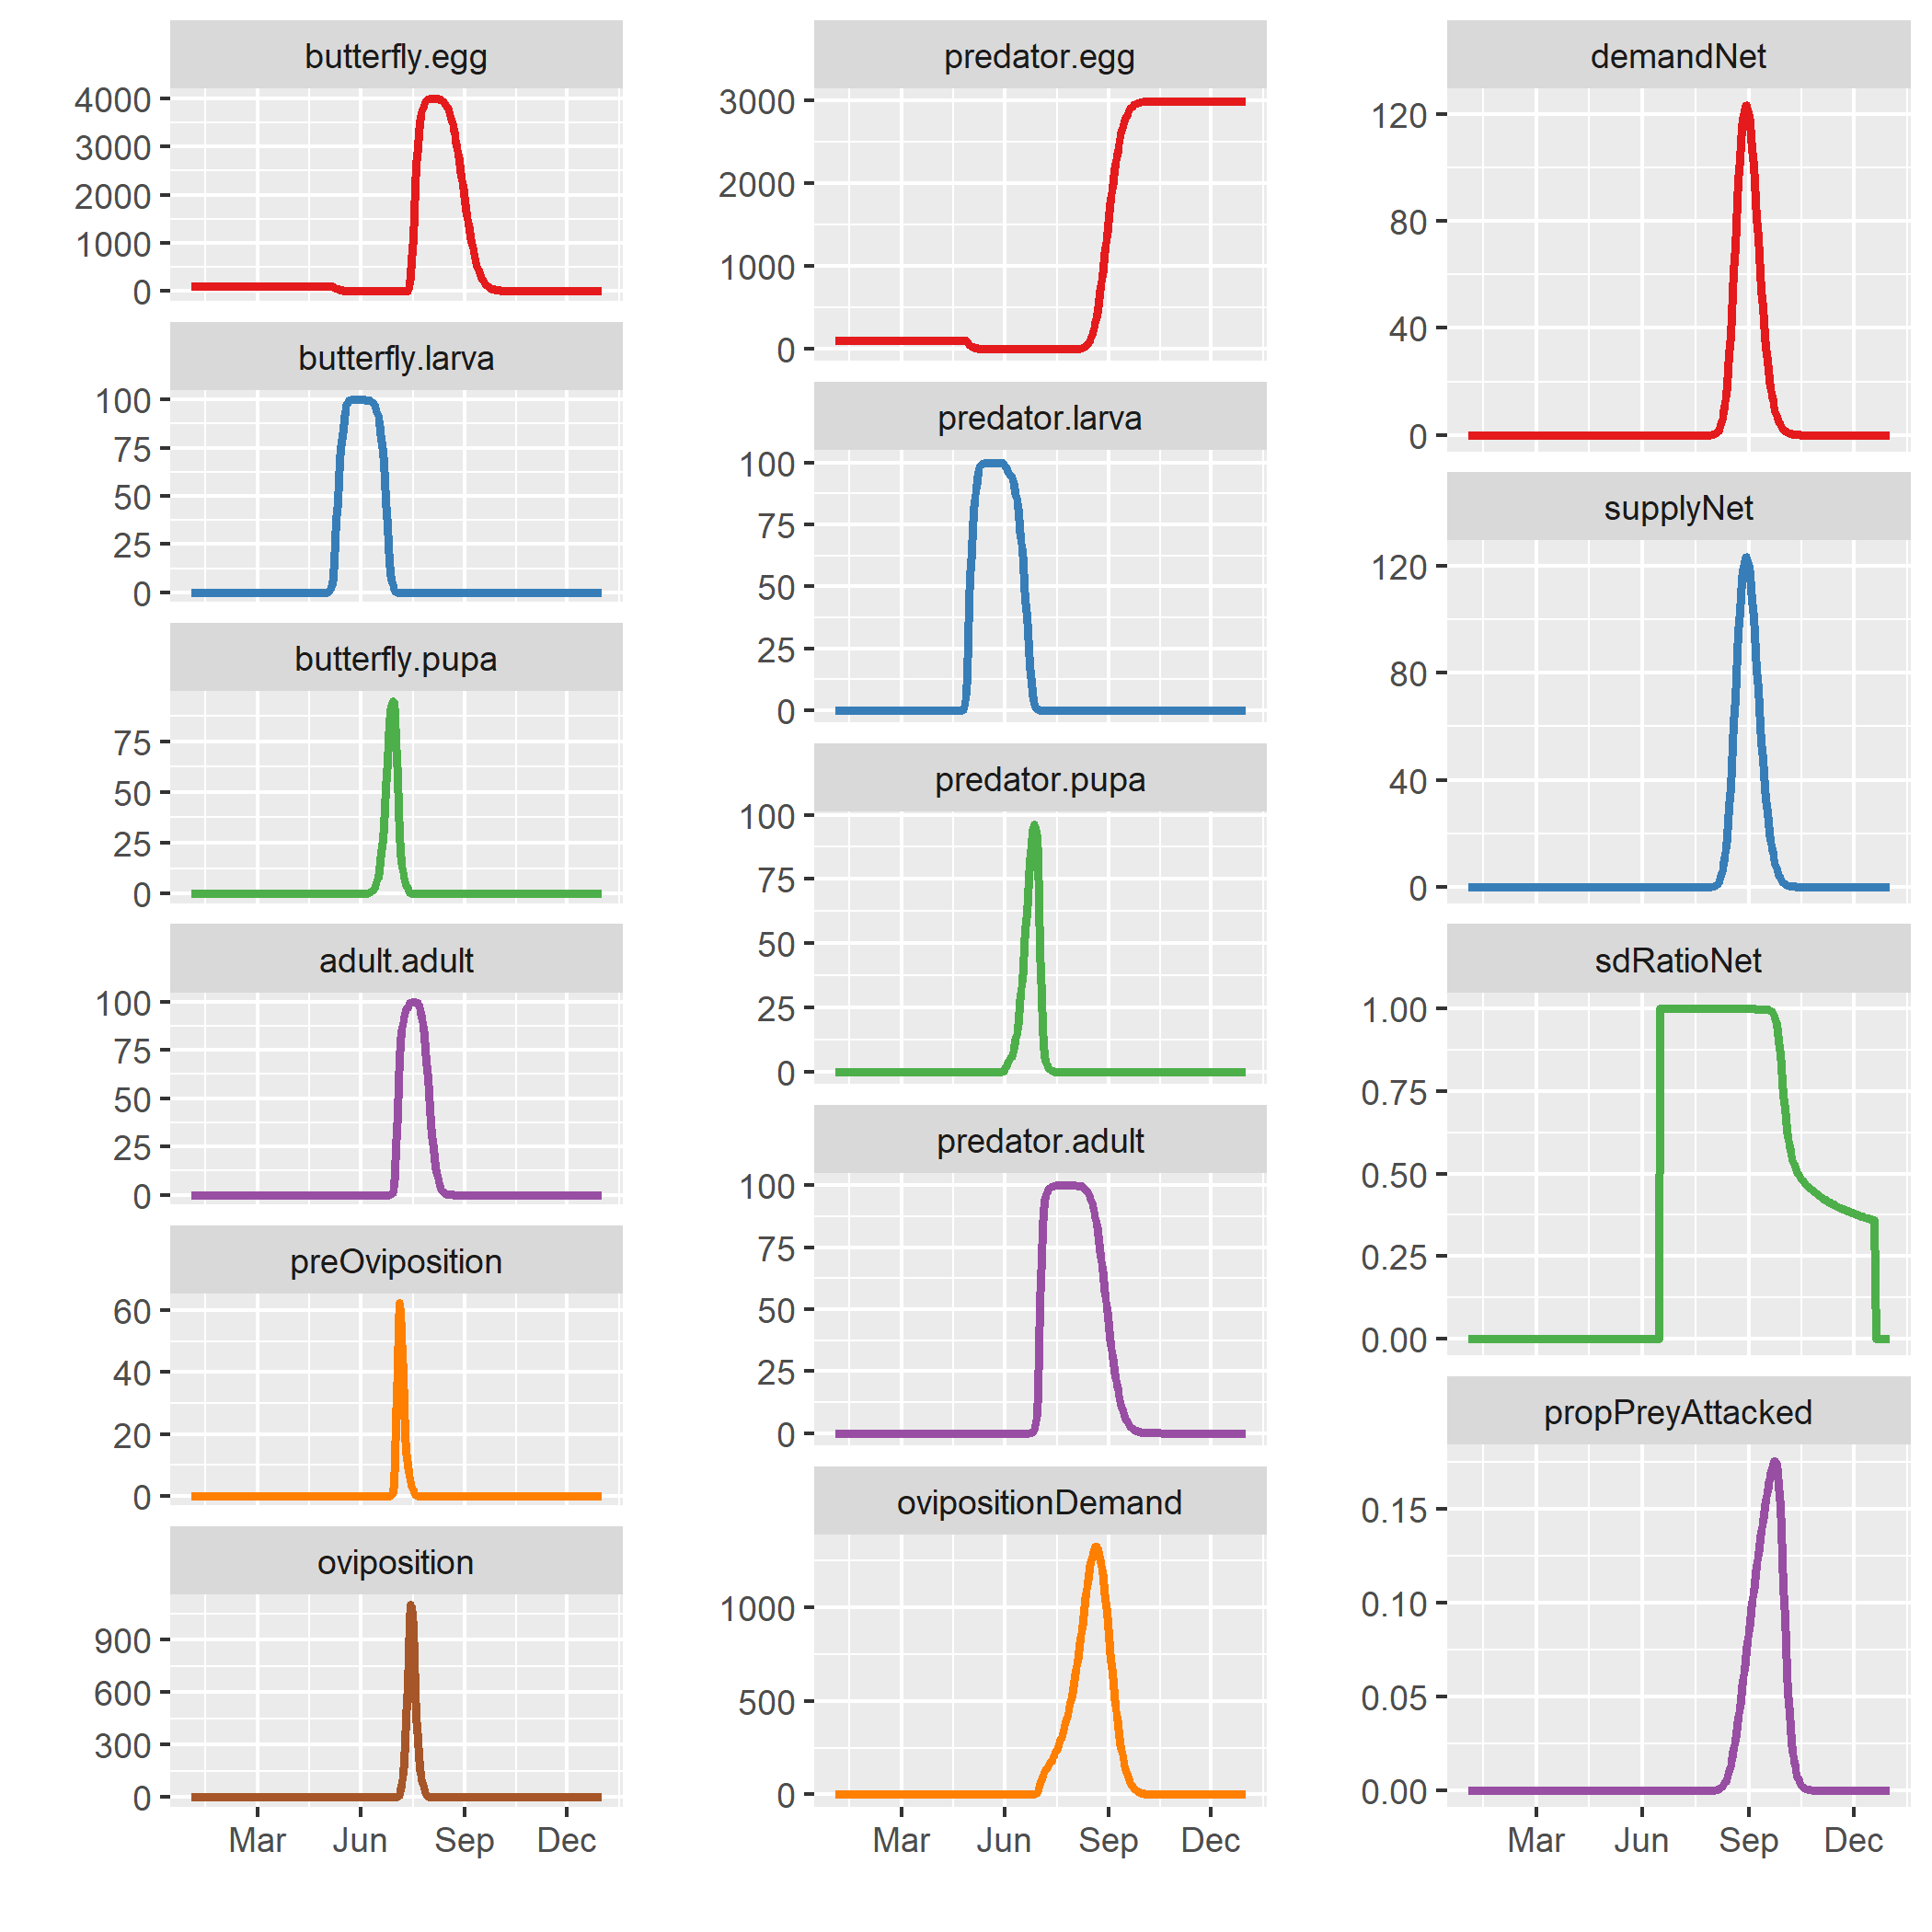
\includegraphics[width=0.9\textwidth]{graphics/func-resp-pred-prey}
\caption{Predator-prey population dynamics. Produced by the \filename{\inputfolder/book/func-resp/func-resp-pred-prey.box}} script.
\label{fig:func-resp-pred-prey}
\end{figure}

\FloatBarrier
\subsection{Parasitoid-host}
\label{ch:trophics-parasitoid-host}
In this example we replace the egg predator in the previous example with a larval parasitoid:

\lstset{numbers=left}
\begin{boxscript}
// func-resp-para-host.box
Simulation sim {
  .steps = 365
  :
  Box butterfly {
    Stage egg {
    :
    }
    Stage larva {
      .inflow = ../egg[outflow]
      .duration = 200
      .timeStep = ./time[step]
      .instantLossRate = 
         parasitoid/funcResp[propHostsAttacked]
      :
    }
    Stage pupa {
    :
    }
    Box adult {
    :
    }
  }
  Box parasitoid {
    +initialAdults = 5
    +adultduration = 90
    Stage egg {
      .inflow = ../funcResp[hostsAttacked]
      .duration = 140
      .timeStep = ./time[step]
      :
    }
    Stage larva {
    :
    }
    Stage pupa {
    :
    }
    Stage adult {
      .initial  = ..[initialAdults]
      .duration = ..[adultduration]
      .inflow   = ../pupa[outflow]
      .timeStep = ./timeStep[value]
      OnOff timeStep { 
        .x = calendar[dayOfYear]
        .xOn = 0 
        .xOff = 180
        .valueOn = 1
        .valueOff = 0
      }
    }
    Stage ovipositionDemand {
      .initial  = ..[initialAdults]
      .duration = ..[adultduration]
      .inflow   = ../pupa[outflow]
      .timeStep = ../adult/timeStep[value]
      .growthFactor = 30
    }
    SuperFunctionalResponse funcResp {
      .attacker = ../adult[content]
      .host = butterfly/larva[content]
      .demand = ../ovipositionDemand[outflow]
      .attackRate = 0.8
    }
  }
  OutputR {
  :
  }
}
\end{boxscript}
\lstset{numbers=none}

In comparison with the earlier model, mortality is no longer incured on the egg stage of the butterfly but rather on the larval stage (lines 13-14). Like before, the loss rate is computed by a functional response model (\code{funcResp} box) but this time the
super functional response model is applied (lines 59-64), since we assume that this parasitoid will super-parasitise. The \code{funcResp} model provides the \code{propHostsAttacked} output which signifies the proportion of hosts lost to parasitisation.

For the parasitoid, the number of eggs laid (line 28) also depends on the outcome of the super functional response model (lines 59-64) but in terms of the number of hosts attacked (line 28), since we assume that only one parasitoid will emerge from a host in case of super-parasitism. In \code{funcResp}, butterfly larvae enter as hosts (line 61). To achieve a somewhat realistic life cycle of the parasitoid, it is assumed to overwinter in the adult stage (lines 39-51). We keep the butterfly's habit from the previous model of overwintering in the egg stage. 

The parasitoid-host model is simpler than the predator-prey model because it entails no energy budget to specify supplies and demands. However, for parasitoids that are host-feeding an energy budget would need to be included.

\begin{figure} [h]
\centering
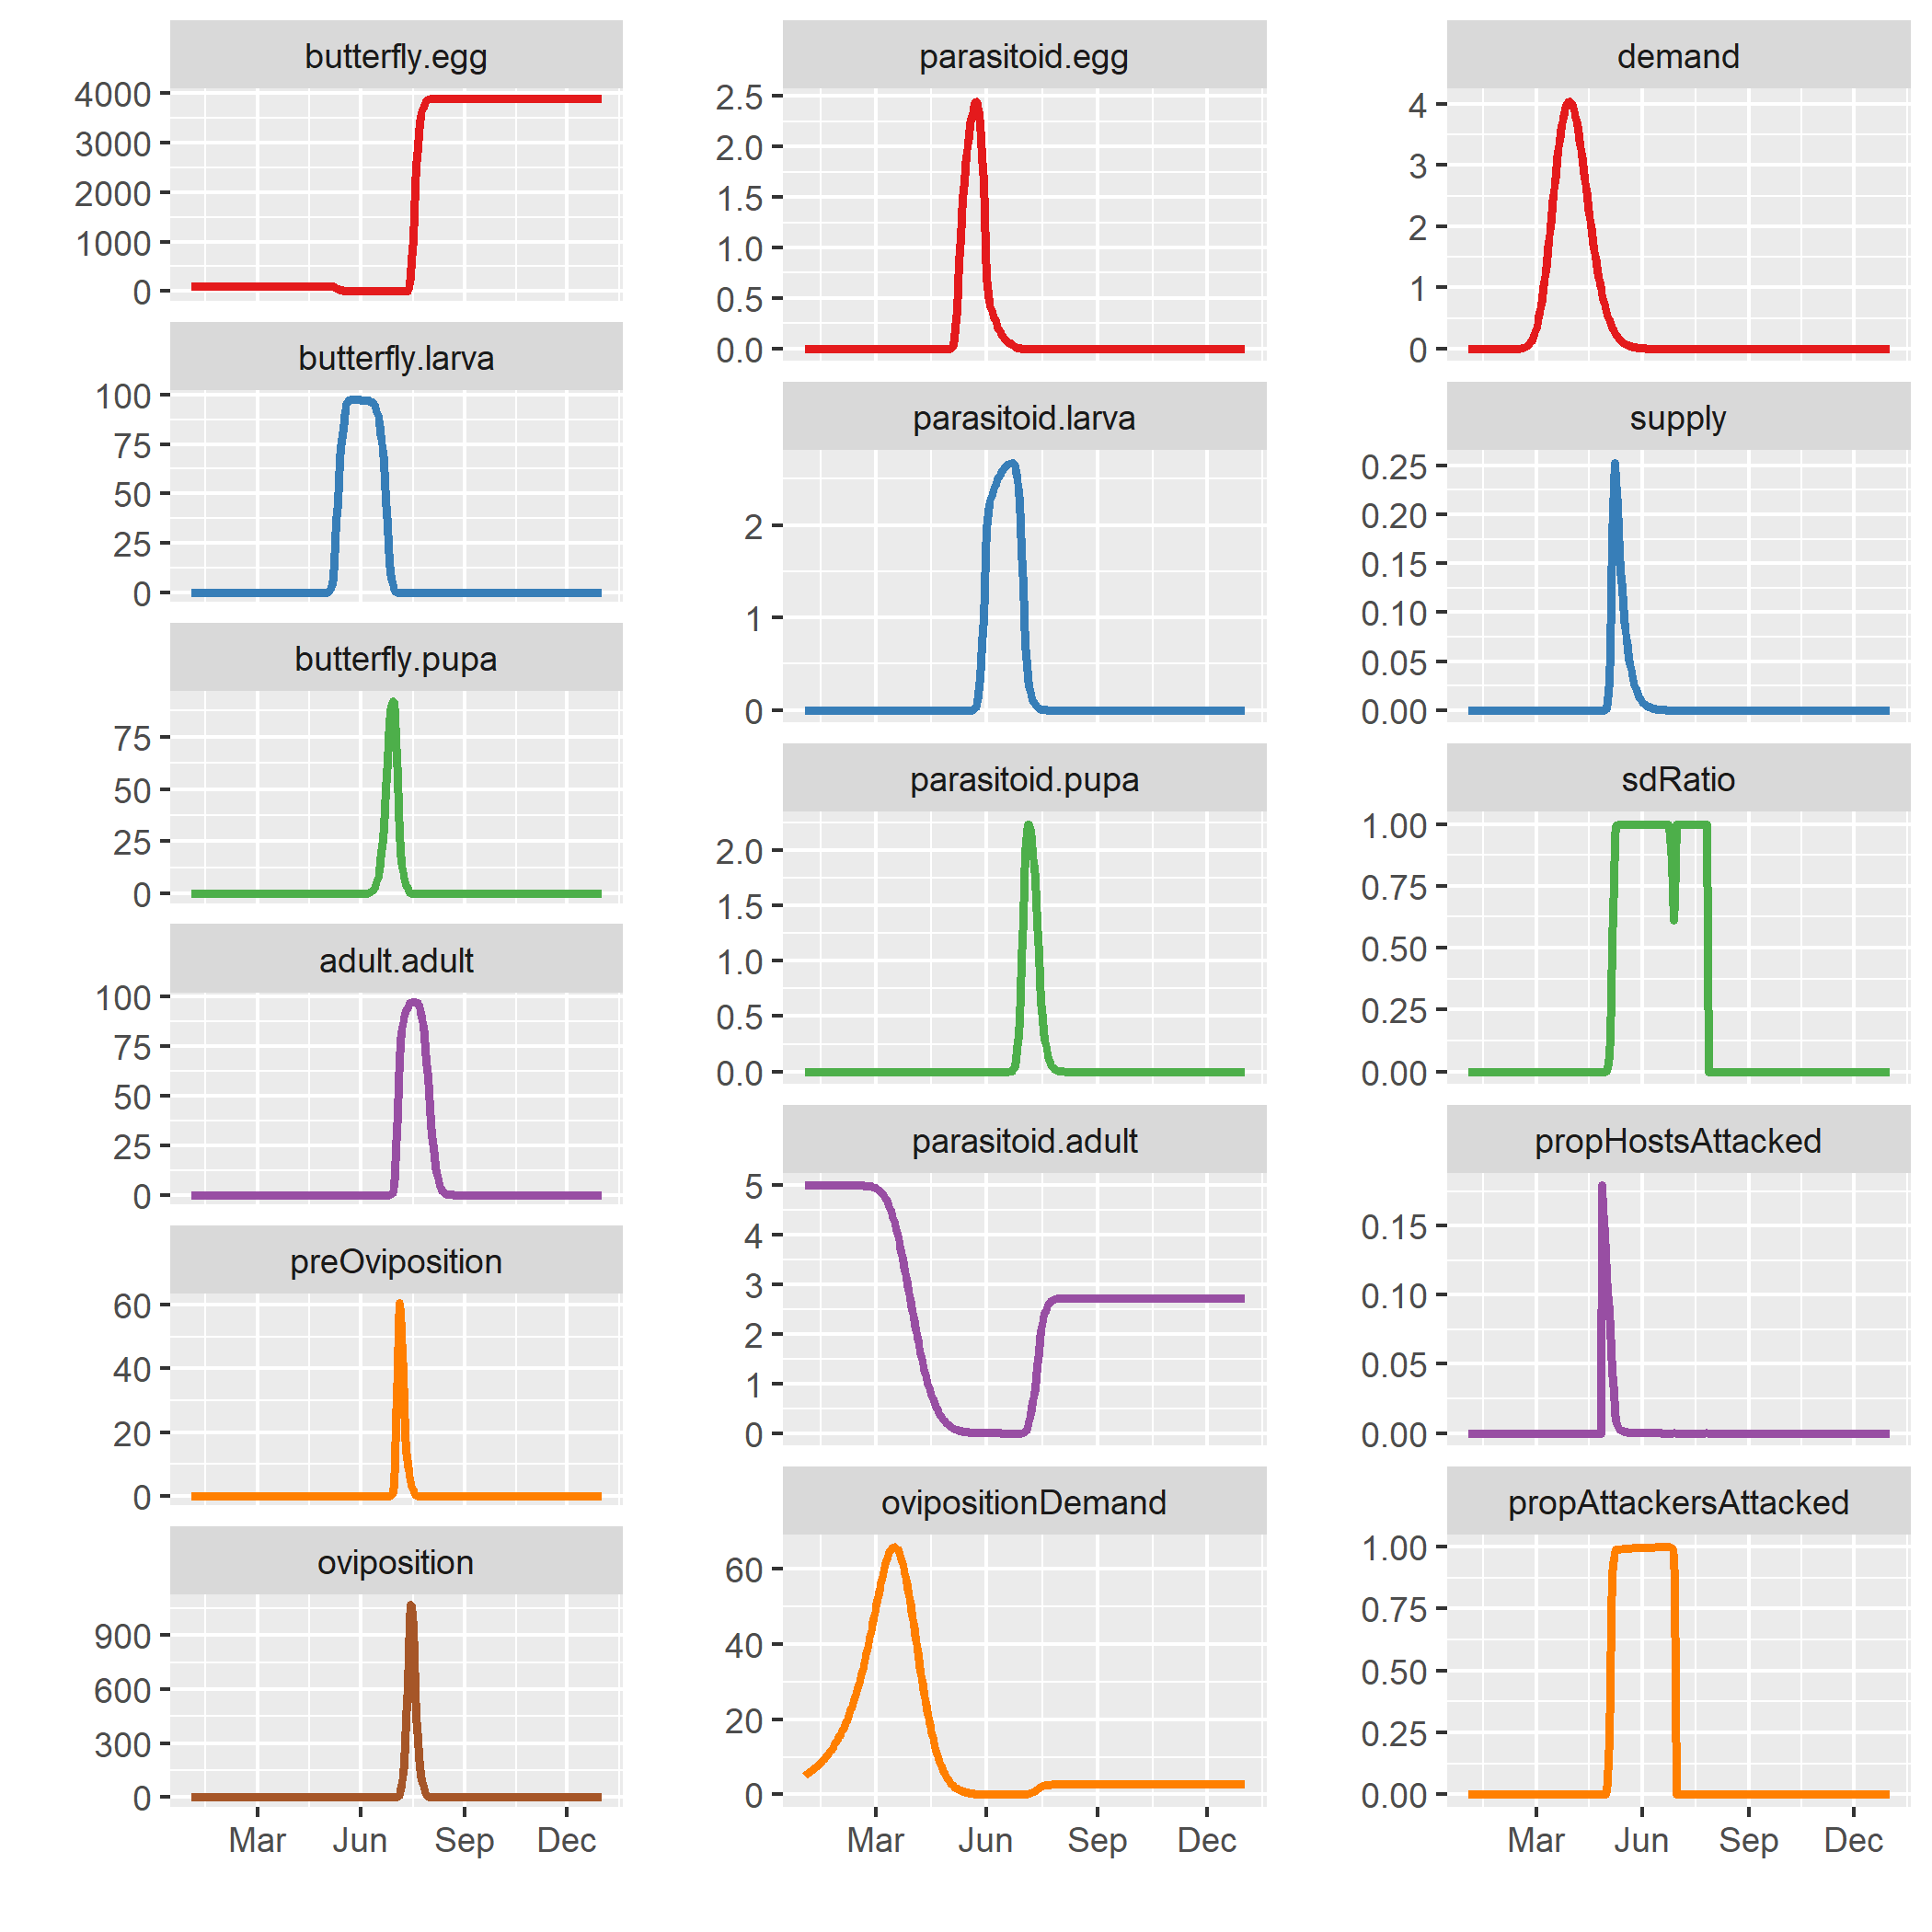
\includegraphics[width=0.9\textwidth]{graphics/func-resp-para-host}
\caption{Parasitoid-host population dynamics. Produced by the \filename{\inputfolder/book/func-resp/func-resp-para-host.box} script.}
\label{fig:func-resp-para-host}
\end{figure}

The output shows that the 5 parasitoids in the beginning of the year have turned into 2.73 parasitoids at the end of the year (\iref{fig:func-resp-para-host}). Thus their demand to lay $24\times 30=150 \text{ eggs}$ (\cf\ lines 5 and 56 in the script) was far from fulfilled . The reason is that the phenology of parasitoid and host restricts the parasitoid to lay eggs in the overwintering eggs of the host only, of which there were only 100 (the initial egg number for the butterfly).

We can now do the math and see how things add up: 100 butterfly eggs turned into 2.73 parasitoids and 97.27 butterflies. These butterflies produced $97.26\times 40=3,891 \text{ eggs}$ (as butterfly fecundity was 40). These numbers were acquired by the simulation output seen in the figure and more precisely at the R prompt by typing \code{tail(sim)}.


% \section{Multiple interactions}
% \label{ch:trophicmultiple}
% \subsection{Many attackers-one resource}

% When many attackers (predators or parasitoids, maybe both) share the same resource (prey or host), more than one density ($Y_i$) and attack rate ($\alpha_i$) enter the functional response model (\iref{fig:trophic-web-1}). We must formulate the model to ensure that the pooled search rate ($s_+$) of all predators does not exceed 1. We achieve this by extending \eqref{eq:lotvol2} thus

% \begin{equation}
% s_+ = 1-exp\left(-\sum \alpha_i Y_i \Delta t\right) \label{eq:searchratemany}
% \end{equation}

% As a first approximation of the predator-specific search rates ($\widetilde{s_i}$), we concur with \eqref{eq:lotvol2}:

% \begin{equation}
% \widetilde{s_i} = 1-exp(-\alpha_i Y_i \Delta t) \label{eq:searchrateapprox}
% \end{equation}

% The attackers are in competition for the common resource ($X$), whereby the actual search rates ($s_i$) will be reduced ($s_i \leq \widetilde{s_i}$). Moreover the actual search rates must add up to the pooled search rate, $\sum s_i = s_+$. We achieve this by splitting the pooled search rate among the predators in proportion to the first approximation:

% \begin{equation}
% s_i = \frac {\widetilde{s}_i} {\sum\widetilde{s}_i} s_+ \label{eq:searchrateprop}
% \end{equation}

% \begin{figure} [ht]
% \centering
% 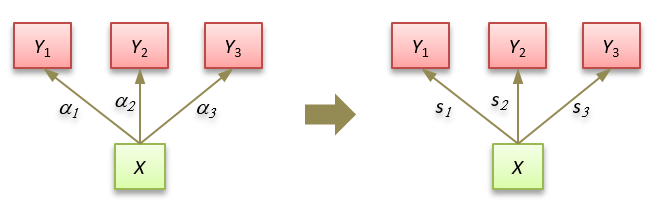
\includegraphics[width=.9\textwidth]{graphics/trophic-web-1}
% \caption{Three attackers ($Y_i$) share a common resource ($X$). Their specific attack rates ($\alpha_i$) are turned into search rates ($s_i$) by \cref{eq:searchratemany,eq:searchrateapprox,eq:searchrateprop}.} 
% \label{fig:trophic-web-1}
% \end{figure}

% Note that \cref{eq:searchratemany,eq:searchrateapprox,eq:searchrateprop} are neutral in two ways. First, if there is only one attacker, they reduce to \cref{eq:lotvol2}. Second, if you split a single predator population ($Y_{single}$) into many ($Y_{single} = \sum Y_i$), all with the same attack rate ($\alpha_{single}=\alpha_i$ for all $i$), then then pooled search rate for the split attacker population will be the same as for the original, single attacker population, $s_{single} = s_+ = \sum s_i$.

% \subsection{One attacker-many resources}
% When an attacker ($Y$) has many resources ($X_j$), it acquires supplies towards fulfilling its demand from all of them (\iref{fig:trophic-web-2}). Yet we must assure that the total amount of prey killed (or hosts parasitized) ($-\Delta X_+$) does not exceed its demand ($\Delta D$). 

% For this purpose we extend \cref{eq:funcresp}, however, noticing a complication, as this functional response equation is meant to work in collaboration with the energy budget for demand and supply in \cref{eq:demandbudget,eq:supplybudget}. In the context of multiple trophic interactions, we must extend \cref{eq:funcresp} in a similar way. 

% Hence, we add gain ($\gamma_j$) to the model, which is the gain  obtained by killing one prey (\eg\ in \si{\milli\gram}). For a parasitoid, we would have $\gamma_j=1$ in the simple case when one host attacked means one parasitoid egg laid. One should be carefull that the units of the attacker demand (\eg\ \si{\milli\gram} or egg-laying rate) match those of $\gamma_j$: 

% \begin{equation}
% -\Delta X_+ = \Delta D \left[1-exp\left(-\frac{\sum s_j \gamma_j X_j}{\Delta D}\right)\right] \label{eq:supplymany}
% \end{equation}

% As a first approximation of the amount killed of each prey ($-\widetilde{\Delta X}_j$), we use \cref{eq:funcresp} directly, except for the added $\gamma_j$ parameter:

% \begin{equation}
% -\widetilde{\Delta X}_j = \Delta D \left[1-exp\left(-\frac{s_j \gamma_j X_j}{\Delta D}\right)\right] \label{eq:supplyapprox}
% \end{equation}

% Next, the total amount of prey killed or hosts parasitised is split in proportion to the first approximation:

% \begin{equation}
% -\Delta X_j = -\frac{\widetilde{\Delta X}_j} {\sum \widetilde{\Delta X}_j} \Delta X_+ \label{eq:supplyprop}
% \end{equation}

% \begin{figure} [ht]
% \centering
% 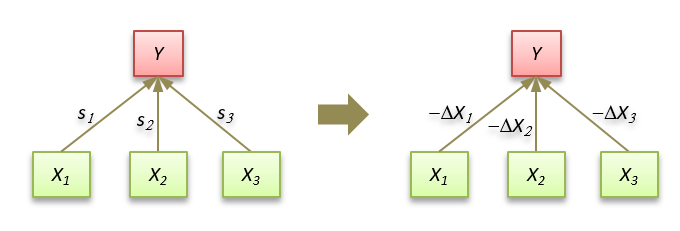
\includegraphics[width=.9\textwidth]{graphics/trophic-web-2}
% \caption{One attacker ($Y$) with many resources ($X_j$). The specific search rates ($s_j$) are turned into resource acquisition rates ($-\Delta X_j$) by \cref{eq:supplymany,eq:supplyapprox,eq:supplyprop}.} 
% \label{fig:trophic-web-2}
% \end{figure}

% \subsection{Many attackers-many resources: a food web}
% \label{ch:trophics-food-web}
% The rationale developed above can be used directly, when many attackers interact with many resources. No special treatment needs to be given to populations acting both as an attacker and a resource, for cannibalism or for mutual predation. We will use a three attacker-two resources system as an example to assist our thinking (\iref{fig:trophic-web-3}).

% To compute the six resource acquisition rates ($-\Delta X_{ij}$), we first apply \cref{eq:searchratemany,eq:searchrateapprox,eq:searchrateprop} to each resource ($X_1$ and $X_2$) separately. This results in the six search rates ($s_{ij}$). These are then applied in \cref{eq:supplymany,eq:supplyapprox,eq:supplyprop} for each attacker ($Y_1$, $Y_2$ and $Y_3$) separately, applying the specific gain rates ($\gamma_{ij}$). This whole procedure gives us the six specific loss rates ($-\Delta X_{ij}$).

% \begin{figure} [ht]
% \centering
% 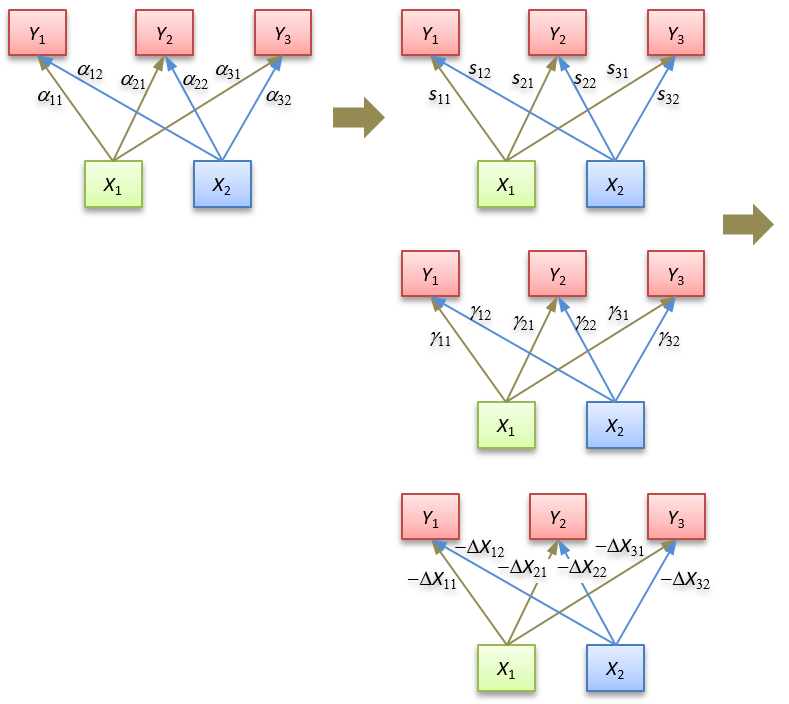
\includegraphics[width=.9\textwidth]{graphics/trophic-web-3}
% \caption{Three attackers ($Y_i$) share two common resources ($X_j$). The specific attack rates ($\alpha_{ij}$) are turned into search rates ($s_{ij}$) and then, by combination with the gain rates ($\gamma_{ij}$), turned into resource acquisition rates ($\Delta X_{ij}$) by \cref{eq:websearchratemany,eq:websearchrateapprox,eq:websearchrateprop,eq:websupplymany,eq:websupplyapprox,eq:websupplyprop1,eq:websupplyprop2}.} 
% \label{fig:trophic-web-3}
% \end{figure}

% Before we attempt an implementation of this whole procedue in \CPP, let's try first it out in an R script (\filename{\inputfolder/book/food-web/food-web.R}) doing the calculations for the system in \iref{fig:trophic-web-3} with some out-of-the-blue parameter settings. First we define a matrix \code{A} with all the attack rates ($\alpha_{ij}$):

% \begin{rscript}
% > A
   % Y1 Y2 Y3   X1   X2
% Y1  0  0  0 0.04 0.04
% Y2  0  0  0 0.07 0.03
% Y3  0  0  0 0.01 0.08
% X1  0  0  0 0.00 0.00
% X2  0  0  0 0.00 0.00
% \end{rscript}

% We keep attackers in rows ($i$) and resources ($j$) in the columns. To achieve generality, all five populations appear in both roles whereby the matrix becomes quadratic. Attack rates on the diagonal would mean cannibalism. 

% Then we set up a matrix \code{G} for the gain rates ($\gamma_{ij}$),
% \begin{rscript}
% > G
   % Y1 Y2 Y3  X1  X2
% Y1  0  0  0 1.0 1.0
% Y2  0  0  0 2.5 4.7
% Y3  0  0  0 2.5 4.7
% X1  0  0  0 0.0 0.0
% X2  0  0  0 0.0 0.0
% \end{rscript}

% Here we assume that \code{Y1} is a parasitoid which lays one egg in each host attacked ($\gamma_{ij}=1$), whereas \code{Y2} and \code{Y3} are predators which both gains \SI{2.5}{\milli\gram} from each \code{X1} prey attacked and \SI{4.7}{\milli\gram} from each prey \code{X2} attacked. Hence \code{X1} and \code{X2} play different roles (host or prey) for different attackers (parasitoid or predator).

% We set the \emph{per capita} demand rates (\code{d}) aware that their units must match the units of the gain rates:
% \begin{rscript}
% > d
     % d
% Y1 0.6
% Y2 5.8
% Y3 2.9
% X1 0.0
% X2 0.0
% \end{rscript}
% \noindent In this case, the parasitoid has an egg laying demand of \SI{0.6}{\per\day} and the two predators have demands of \SI{5.8}{\milli\gram\per\day} and \SI{2.9}{\milli\gram\per\day}, respectively.

% The population densities are kept in the vector \code{N}: 

% \begin{rscript}
% > N
% Y1 Y2 Y3 X1 X2 
 % 5 10  2 15 20 
% \end{rscript}

% \noindent By multiplying population densities with demand rates and assuming a time step of \SI{1}{d}, we arrive at the population-wise demands:

% \begin{rscript}
% >   D
      % D
% Y1  3.0
% Y2 58.0
% Y3  4.8
% X1  0.0
% X2  0.0
% \end{rscript}

% \noindent Thus \code{D} contains the demand of each attacker population  $i$ ($\Delta D_i$).

% Next, \cref{eq:searchratemany,eq:searchrateapprox,eq:searchrateprop,eq:supplymany,eq:supplyapprox,eq:supplyprop} are implemented one by one, slightly extended for multiple interactions. We calculate the pooled search rates $s_+$ in \cref{eq:searchratemany} for each population in the role as a resource ($j$), \ie,

% \begin{equation}
% s_{+j} = 1-exp\left(-\sum\limits_{i}\alpha_{ij}N_i \Delta t\right) \label{eq:websearchratemany}
% \end{equation}

% \noindent from which we get
% \begin{rscript}
% > round(s_pooled,3)
   % Y1    Y2    Y3    X1    X2 
% 0.000 0.000 0.000 0.601 0.483 
% \end{rscript}

% \noindent whereby the pooled search rate for resources \code{X1} and \code{X2} are 0.601 and 0.483 respectively. 

% We calculate the approximate search rates $\widetilde{s_i}$ from \cref{eq:searchrateapprox}. Since this pertains to all attacker $\times$ resource interactions, we end up with a matrix:

% \begin{equation}
% \widetilde{s_{ij}} = 1-exp(-\alpha_{ij} N_i \Delta t) \label{eq:websearchrateapprox}
% \end{equation}

% \noindent Here, it has been amended with the sum for each resource:
% \begin{rscript}
% > round(s_approx_with_sum,3)
    % Y1 Y2 Y3    X1    X2
% Y1   0  0  0 0.181 0.181
% Y2   0  0  0 0.503 0.259
% Y3   0  0  0 0.020 0.148
% X1   0  0  0 0.000 0.000
% X2   0  0  0 0.000 0.000
% Sum  0  0  0 0.704 0.588
% \end{rscript}

% \noindent Note that the summed, approximate search rates are larger than the proper, pooled search rates above, \eg\ for \code{X1}: 0.704 > 0.601. 

% This is what we fix in the final step, calculating the search rates $s_i$ from \cref{eq:searchrateprop} or, rather $s_{ij}$, as we calculate $s_i$ for each resource $j$ attacked by attacker $i$: 

% \begin{equation}
% s_{ij} = \frac {\widetilde{s}_{ij}} {\sum\widetilde{s}_{ij}} s_{+j} \label{eq:websearchrateprop}
% \end{equation}

% \noindent Thus we arrive at the following, again shown with an extra row for the sums:
% \begin{rscript}
% > round(s_with_sum,3)
    % Y1 Y2 Y3    X1    X2
% Y1   0  0  0 0.155 0.149
% Y2   0  0  0 0.430 0.213
% Y3   0  0  0 0.017 0.121
% X1   0  0  0 0.000 0.000
% X2   0  0  0 0.000 0.000
% Sum  0  0  0 0.601 0.483
% \end{rscript}
% \noindent To wit the summed search rates match the proper, pooled search rates ($s_{+j}$) precisely.

% We use the search rates $s_{ij}$ to calculate the total amount acquired by each attacker $-\Delta X_+$ in \cref{eq:supplymany}. For attacker $i$ we get the total acquisition from all resources ($j$):

% \begin{equation}
% -\Delta N_{i+} = \Delta D_i \left[1-exp\left(-\frac{\sum\limits_{j} s_{ij} \gamma_{ij} N_j}{\Delta D_i}\right)\right] \label{eq:websupplymany}
% \end{equation}

% \noindent Here it is shown together with the demands (\code{D}) for comparison:

% \begin{rscript}
% > round(mDX_pooled_with_D,2)
     % mDX    D
% Y1  2.49  3.0
% Y2 26.89 58.0
% Y3  4.41  4.8
% X1  0.00  0.0
% X2  0.00  0.0
% \end{rscript}
% \noindent If you compare the amounts acquired ($-\Delta N_{i+}$ or \code{mDX} in R) with the population demands ($D_i$ or \code{D} in R), you can check that $-\Delta N_{i+} < D_i$ holds for all $i$; \ie\ no attacker acquires resources above its demand.

% Next we calculate the approximate acquisitions rates, $-\widetilde{\Delta X}_j$ from \cref{eq:supplyapprox}, for each attacker ($i$): 

% \begin{equation}
% -\widetilde{\Delta N}_{ij} = \Delta D_i \left[1-exp\left(-\frac{s_{ij} \gamma_{ij} N_j}{\Delta D_i}\right)\right] \label{eq:websupplyapprox}
% \end{equation}

% \noindent This results in a matrix showing the first approximation of the amount acquired by each attacker. We add a column to show the total approximate acquisition by each attacker:
% \begin{rscript}
% > round(mDX_approx_with_sum, 2)
   % Y1 Y2 Y3    X1    X2   Sum
% Y1  0  0  0  1.62  1.89  3.50
% Y2  0  0  0 14.07 16.92 30.99
% Y3  0  0  0  0.59  4.35  4.95
% X1  0  0  0  0.00  0.00  0.00
% X2  0  0  0  0.00  0.00  0.00
% \end{rscript}
% \noindent We notice that from this we get a total acquisition for each attacker, that exceeds the proper pooled resource acquisition ($-\Delta N_{i+}$) above. 

% We hurry to fix this in the final and sixth step of the procedure, calculating both the supply to each attacker $j$ from each resource $i$ ($\Delta S_{ij}$) and the loss from each resource $i$ to each attacker $j$ ($\Delta N_{ij}$). Based on \cref{eq:supplyprop}, we get

% \begin{equation}
% \Delta S_{ij} = -\frac{\widetilde{\Delta N}_{ij}} {\sum\limits_{j} \widetilde{\Delta N}_{ij}} \Delta N_{i+} \label{eq:websupplyprop1}
% \end{equation}

% \begin{equation}
% -\Delta N_{ij} = -\frac{\Delta S_{ij}}{\gamma_{ij}} \label{eq:websupplyprop2}
% \end{equation}

% Here, the supply matrix $\Delta S_{ij}$ has been extended with the total supply to each attacker together with its demand:
% \begin{rscript}
% > round(S,2)
   % Y1 Y2 Y3    X1    X2 Supply    D
% Y1  0  0  0  1.15  1.34   2.49  3.0
% Y2  0  0  0 12.21 14.68  26.89 58.0
% Y3  0  0  0  0.53  3.88   4.41  4.8
% X1  0  0  0  0.00  0.00   0.00  0.0
% X2  0  0  0  0.00  0.00   0.00  0.0
% \end{rscript}

% \noindent We check the output and find that, indeed, for each attacker the total supply (\code{Supply}) does not exceed the demand (\code{D}). In a food web model the supply would go into each predator's energy budget \cref{eq:supplybudget} and spent towards meeting one or more demands: respiration, reproduction or growth.

% The losses $\Delta N_{ij}$ which should be subtracted from the population densities $N_j$ are
% \begin{rscript}
% > round(mN,2)
     % Y1 Y2 Y3    X1    X2
% Y1    0  0  0  1.15  1.34
% Y2    0  0  0  4.88  3.12
% Y3    0  0  0  0.21  0.83
% X1    0  0  0  0.00  0.00
% X2    0  0  0  0.00  0.00
% Loss  0  0  0  6.24  5.29
% N     5 10  2 15.00 20.00
% \end{rscript}
% \noindent Again, we check the output and find that the losses (row \code{Loss}) do not exceed the population densities (row \code{N}).

% \subsection {Implementation in the \code{FoodWeb} class} 
% The food web algorithm described above was implemented in the \code{FoodWeb} class. The \filename{\inputfolder/food-web/food-web-1.box} script repeats the calculations above and was written just to test that the R code and the \CPP\ implementation are equivalent. If you run that script and then type \code{sim} at the R prompt to display all the output, you can verify that the numbers match with those above.

% The \filename{\inputfolder/food-web/food-web-2.box} script provides an example how to use \code{FoodWeb} to model three interacting populations: \code{butterfly}, \code{trichogramma} and \code{carabus}. The egg stage of the butterfly serves both as a host for the parasitoid and as prey for the predator. Butterfly larvae are prey as well.

% A \code{FoodWeb} box  takes the matrices $\alpha_{ij}$ and $\gamma_{ij}$ and the time step $\Delta t$ as input. The matrices are provided in a text file each, \code{attackFile} and \code{gainFile}, as can be seen in lines 3-4 in this excerpt from the box script:

% \lstset{numbers=left}
% \begin{boxscript}
% // From food-web-2.box
% FoodWeb web {
  % .attackFile = "food-web-2-attack-matrix.txt"
  % .gainFile   = "food-web-2-gain-matrix.txt"
  % .showMatrices = TRUE
  % FoodWebBox butterflyEgg {
    % .density = butterfly/egg[content]
  % }
  % FoodWebBox butterflyLarva {
    % .density = butterfly/larva[content]
  % }
  % FoodWebBox trichogrammaAdult {
    % .density = trichogramma/adult/individuals[content]
    % .demand  = trichogramma/adult/oviposition[outflow]
  % }
  % FoodWebBox carabusAdult {
    % .density = carabus/adult/individuals[content]
    % .demand  = carabus/adult/oviposition[outflow]
  % }
% }
% \end{boxscript}
% \lstset{numbers=none}

% The \filename{food-web-2-attack-matrix.txt} file contains all the $\alpha_{ij}$ values:

% \begin{textfile}
% web/butterflyEgg web/butterflyLarva%\brk%web/trichogrammaAdult web/carabusAdult
% 0 0 0 0
% 0 0 0 0
% 0.01 0 0 0
% 0.005 0.02 0 0
% \end{textfile}

% The column labels refer to the nodes in the food web which are defined as \code{FoodWebBox} boxes in the box script (lines 6-19). They play two roles in the matrix acting both as attackers (rows) and as resources (columns). You can check that the attack rate of the parasitoid on host eggs is 0.01, and that the predator has two prey attacked at rates of 0.005 and 0.02 for prey eggs and larvae, respectively.

% You set up each \code{FoodWebBox} by defining the \code{density} of the pertinent population and, if it is an attacker, its \code{demand} as well (lines 6-19). All three populations are composed as a series of life stages (\code{Stage} boxes) running on day-degree scales. You can study the \filename{food-web-2.box} script to work out the details. If you type \code{list} at the \US\ prompt, you can see the structure of the whole model. Here we focus on the \code{FoodWeb} box only.

% The \filename{food-web-2-gain-matrix.txt} file contains all the $\gamma_{ij}$ values:

% \begin{textfile}
% web/butterflyEgg web/butterflyLarva%\brk%web/trichogrammaAdult web/carabusAdult
% 0 0 0 0
% 0 0 0 0
% 1 0 0 0
% 0.7 10 0 0
% \end{textfile}

% It can be seen that for every host egg attacked, one parasitoid egg is laid ($\gamma=1$), while for the predator there is a conversion cost of 30\% ($\gamma=0.7$). One prey larva provides enough food to produce 10 predator eggs.

% A \code{FoodWebBox} is equipped with four inputs, in addition to \code{density} and \code{demand}. These four inputs are kept updated automatically by the \code{FoodWeb} box (by use of the complete works of equations described above):

% \begin{description}
  % \item[\code{supply}] \hfill \\ Supply to the \code{FoodWebBox}
  % \item[\code{loss}] \hfill \\ Loss from the \code{FoodWebBox}
  % \item[\code{supplyDemandRatio}] \hfill \\ The supply/demand ratio (zero if demand is zero)
  % \item[\code{lossRatio}] \hfill \\ The loss/density ratio (zero if density is zero)
% \end{description}

% \begin{figure} [hb]
% \centering
% \includegraphics[width=\textwidth]{graphics/food-web-2}
% \caption{Ten years of food web dynamics shown as the daily rates of loss and supply for two hosts/prey (butterfly eggs and larvae), a parasitoid and a predator. Produced by the \filename{food-web/food-web-2.box} script.}
% \label{fig:food-web-2}
% \end{figure}

% The boxes that you refer to by the column headings in \filename{attackFile} and \filename{gainFile} must have those six input ports. The \code{FoodWebBox} class is provided for this purpose. It can be used directly as shown above (lines 6-19), or you can derive your own class from it (in \CPP), if you need more functionality.

% Reading through the \filename{food-web/food-web-2.box} script, you can see how losses and supplies, administered by the \code{web} box, are applied:

% \lstset{numbers=left}
% \begin{boxscript}
% :
% Box butterfly {
  % Stage egg {
    % :
    % .instantLossRate = web/butterflyEgg[lossRatio]
  % }
  % Stage larva {
    % :
    % .instantLossRate = web/butterflyLarva[lossRatio]  
  % }
% :
% Box trichogramma {
  % Stage juvenile {
    % .inflow = web/trichogrammaAdult[supply]
    % :
  % }
% }
% :
% Box carabus {
  % Stage egg {
    % .inflow = web/carabusAdult[supply]   
    % :
  % }
% }
% :
% \end{boxscript}
% \lstset{numbers=none}

% Other tricks you will encounter in this box script are density-dependent survival of butterfly and carabus larvae, winter kill of most parasitoids and an age increment for parasitoids and predators that depends on food supply (the animals age more slowly with decreasing supply/demand ratio.).
